\documentclass[Master,ngerman,UKenglish]{scrbook}
%------------------------------------------------------------------------------
% This file contains a skeleton thesis for
% a Physics or Astronomy Institute in the University of Bonn

% Specify the thesis type as an option: PhD, Master, Diplom, Bachelor
% Specify the thesis stage as an option: Draft (default), Submit, Final, PILibrary

% Specify the language(s) in the class and then use babel.
% If you need more than one language, give the default language last,
% e.g. ngerman,UKenglish for a thesis in British (UK) English where you want
% to be able to set the language to German for some part of it.

%------------------------------------------------------------------------------
% Pass TeX Live version to the package
% Use command pdflatex --version to find out which version you are running
% Add option backref=false when your thesis is ready to turn off back-referencing
% in your bibliography
\usepackage[texlive=2016,biblatex=false,newtx=false,txfonts=true]{ubonn-thesis}
% Adjustments to standard biblatex style
% \usepackage{ubonn-biblatex}

% Glossary package
% \usepackage[acronym,toc,nosuper]{glossaries}
% TikZ packages and libraries
% \usepackage{tikz}
% \usepackage{tikz-3dplot}
% \usepackage{pgfplots}
% \usetikzlibrary{positioning,shapes,arrows}
% \usetikzlibrary{decorations.pathmorphing}
% \usetikzlibrary{decorations.markings}
\usepackage{thesis_defs}
\usepackage{todonotes}
\usepackage{amsmath}
\usepackage{placeins}
%------------------------------------------------------------------------------
% Instead of colouring  links, cites, table of contents etc.
% put them in a coloured box for the screen version.
% This is probably a good idea when you print your thesis.
\hypersetup{colorlinks=false,
  linkbordercolor=blue,citebordercolor=magenta,urlbordercolor=darkgreen
}

%------------------------------------------------------------------------------
% When writing your thesis it is often helpful to have the date and
% time in the output file. Comment this out for the final version.
% \ifoot[\today{} \thistime]{\today{} \thistime}

% In order to check if your labels are referenced try the refcheck package
% \usepackage{refcheck}

%------------------------------------------------------------------------------
% biblatex is included by ubonn-thesis. Look there for the settings used.
% See the options for settings that can be changed easily.
% For further changes copy the \RequirePackage[...]{biblatex} here
% and include ubonn-thesis with the option biblatex=false.

% Specify the bibliography files here and not at the end!
% Use standard_refs-bibtex if you use bibtex8
% and standard_refs-biber  if you use biber
% \addbibresource{thesis_refs.bib}
% \addbibresource{../refs/standard_refs-biber.bib}

%------------------------------------------------------------------------------
% The following definitions are used to produce the title pages
% needed at various stages
\newcommand{\thesistitle}{Event reconstruction for Dark Photon searches at NA64}
\newcommand*{\thesisauthor}{Srijan Sehgal}
\newcommand*{\thesistown}{Bonn}
\renewcommand*{\InstituteName}{\HISKP}
\renewcommand*{\inInstitute}{\inHISKP}
\renewcommand*{\InstituteAddress}{\HISKPaddress}
% Adjust \thesisreferee...text depending on male/female referee
\newcommand*{\thesisrefereeonetext}{1.\ Gutachter}
\newcommand*{\thesisrefereeone}{Prof.\ Dr.\ Bernhard Ketzer}
\newcommand*{\thesisrefereetwotext}{2.\ Gutachter}
\newcommand*{\thesisrefereetwo}{Prof.\ Dr.\ Jochen Dingfelder}
% Date when thesis was submitted (Master/Diplom)
% Year or Month, Year when thesis was submitted (PhD)
\newcommand*{\thesissubmit}{16.12.2019}
% \newcommand*{\thesissubmit}{Month 2016}
% Date of thesis examination (PhD)
\newcommand*{\thesispromotion}{16.12.2016}
% Month and year of the final printed version of the thesis
\newcommand*{\thesismonth}{December}
\newcommand*{\thesisyear}{2019}
\newcommand*{\thesisnumber}{BONN-IR-2019-XXX}

%------------------------------------------------------------------------------
% The abstract is only needed for the printed version and should be in
% English regardless of the language of the thesis
\newcommand{\thesisabstract}{%
  \begin{otherlanguage}{UKenglish}
    This is your thesis abstract. It may be in a language that is
    different from the rest of your thesis.
  \end{otherlanguage}
}

%------------------------------------------------------------------------------
% \includeonly can be used to select which chapters you want to process
% A simple \include command just inserts a \clearpage before and after the file
% Note that \includeonly can be quite picky! Do not forget to put a
% comma after the filename, otherwise it will simply be ignored!
% \includeonly{%
%   thesis_intro,
%   thesis_appendix,
%   thesis_acknowledge
% }

%------------------------------------------------------------------------------
% Give a list of directories where figures can be found. Do not leave
% any spaces in the list and end the directory name with a /
\graphicspath{%
  {../figs/}%
  {../figs/cover/}%
  {../figs/graphics/}%
  {../feynmf/}%
}

%------------------------------------------------------------------------------
% Make a glossary and a list of acronyms
% \makeglossaries

% Glossary entries
% %
% Contains a list of glossary definitions to illustrate how a glossary
% using the glossaries package
%

\newglossaryentry{siunitx}{name=siunitx,
  description={the best package around for typesetting units}}
\newglossaryentry{csquotes}{name=csquotes,
  description={a very nice package for using consistent quotes that is
  language sensitive}}
\newglossaryentry{LaTeX}{name=\LaTeX,
  description={the typesetting program that is used for this guide}}


\newacronym[plural=CRs,firstplural=cosmic rays (CRs)]{CR}{CR}{cosmic ray}  
\newacronym[plural=UHECRs,firstplural=ultra-high energy cosmic rays (UHECRs)]{UHECR}{UHECR}{ultra-high energy cosmic ray}  
\newacronym{UHE}{UHE}{ultra high energy}
\newacronym{UHEnu}{UHE$\nu$}{Ultra high energy neutrino}
\newacronym{UHEnus}{UHE$\nu$}{ultra high energy neutrinos}
\newacronym{SD}{SD}{Surface Detector}
\newacronym{FD}{FD}{Fluorescence Detector}
\newacronym{HEAT}{HEAT}{High Elevation Auger Telescope}
\newacronym[first= \textit{lateral distribution function} (LDF)]{LDF}{LDF}{lateral distribution function}
\newacronym{EM}{EM}{electromagnetic}
\newacronym{MVA}{MVA}{multivariate analysis}
\newacronym{AUGER}{AUGER}{Pierre Auger Observatory}
\newacronym[plural=EASs,firstplural= Extensive Air Showers (EASs)]{EAS}{EAS}{extensive air shower}
\newacronym{VEM}{VEM}{vertical equivalent muon}
\newacronym{MoPS}{MoPS}{Multiplicity-of-Positive-Steps}
\newacronym{FADC}{FADC}{flash analog-to-digital converter}
\newacronym{GZK}{GZK}{Greisen–Zatsepin–Kuzmi}
\newacronym{ToT}{ToT}{time-over-threshold}
\newacronym{ToTd}{ToTd}{Time-over-Threshold-deconvolved}
\newacronym{DGL}{DG$\mathrm{_{low}}$}{down-going low}
\newacronym{DGH}{DG$\mathrm{_{high}}$}{down-going high}
\newacronym{ES}{ES}{Earth-skimming}
\newacronym{TA}{TA}{Telescope Array}
\newacronym{CNB}{CNB}{Cosmic Neutrino Background}
\newacronym{CMB}{CMB}{Cosmic Microwave Background}
\newacronym{ISM}{ISM}{interstellar medium}
\newacronym{AGN}{AGN}{Active Galactic Nuclei}
\newacronym{eV}{eV}{electronvolts}
\newacronym{HESS}{HESS}{High Energy Stereoscopic System}
\newacronym{CTA}{CTA}{Cherenkov Telescope Array}
\newacronym{EBL}{EBL}{extragalactic background light}
\newacronym{WIMP}{WIMP}{Weakly Interacting Massive Particle} 
\newacronym{CC}{CC}{Charged Current}
\newacronym{NC}{NC}{Neutral Current}
\newacronym{QCD}{QCD}{quantum chromodynamics}
\newacronym{MHz}{MHz}{megahertz}
\newacronym{GHz}{GHz}{gigahertz}
\newacronym{UV}{UV}{ultraviolet}
\newacronym{IACT}{IACT}{Imaging Cherenkov telescope}
\newacronym{PMT}{PMT}{photomultiplier tube}
\newacronym{RD}{RD}{Radio Detector}
\newacronym{UMD}{UMD}{Underground Muon Detector}
\newacronym{CLF}{CLF}{Central Laser Facility}
\newacronym{XLF}{XLF}{eXtreme Laser Facility}
\newacronym{WCD}{WCD}{Water Cherenkov Detector}
\newacronym{VCT}{VCT}{vertically central through-going}
\newacronym{TH}{TH}{threshold trigger}
\newacronym{UUB}{UUB}{upgraded unified board}
\newacronym{ADST}{ADST}{Advanced Data Summary Tree}
\newacronym{AoP}{AoP}{Area over Peak}
\newacronym{MC}{MC}{Monte Carlo}
\newacronym{GDAS}{GDAS}{Global Data Assimilation System}
\newacronym{FDA}{FDA}{Fisher Discriminant Analysis}
\newacronym{LDA}{LDA}{Linear Discriminant Analysis}
\newacronym{FOV}{FOV}{field of view}





% Draft version - add DRAFT to header.
% You can use draftwatermark to add DRAFT to the cover page.
% Note that this only works if \unitlength is set to 1pt.
% This is normally not the case - it is set to 1mm in ubonn-thesis.sty.
% The background package is used for later versions of TeX Live.
%\setlength{\unitlength}{1pt}
% \ifthenelse{\equal{\ThesisVersion}{Draft}}{%
%   \usepackage{background}
%   \ifthenelse{\texlive < 2013}{%
%     \SetBgContents{DRAFT}
%     \SetBgColor{blue!30}
%   }{%
%     \backgroundsetup{contents=DRAFT, color=blue!30}
%   }
% }

%------------------------------------------------------------------------------
\begin{document}

% Cover page of thesis - this is only needed for the printed final
% version to be submitted to the department library
% Do not use this page for thesis submission to the Prüfungsamt or Promotionsbüro!
\ifthenelse{\equal{\ThesisVersion}{PILibrary}}{%
  \typeout{Document \jobname, Info: PI library version of thesis}
  \input{../cover/\ThesisType_Cover}
}{}

% Start counting pages from the title page
\frontmatter
% Dedication has to come before \maketitle
% \dedication{For ...}

% Select the correct title page(s)
\ifthenelse{\equal{\ThesisType}{Unknown}}{%
  \typeout{Document \jobname, Error: Unknown thesis type - no title page printed}
}{%
  % Bachelor thesis only has one title page
  \ifthenelse{\equal{\ThesisType}{Bachelor}}{%
    \typeout{Document \jobname, Info: Bachelor thesis}
    \input{../cover/\ThesisType_Title}
  }{%
    \ifthenelse{\equal{\ThesisVersion}{Final} \OR \equal{\ThesisVersion}{PILibrary}}{%
      % Final and PI library versions
      \typeout{Document \jobname, Info: Final version of a \ThesisType  thesis}
      \input{../cover/\ThesisType_Final_Title}
    }{% Submission and draft versions
      \input{../cover/\ThesisType_Submit_Title}
      \typeout{Document \jobname, Info: Draft/submission version of a \ThesisType  thesis}
    }
  }
}

\pagestyle{scrplain}

%------------------------------------------------------------------------------
% You can add your acknowledgements here - don't forget to also add
% them to \includeonly above
%------------------------------------------------------------------------------
\chapter*{Acknowledgements}
\label{sec:ack}
%------------------------------------------------------------------------------
Even though this thesis has my name on the front a number of people were involved in shaping its final form both in person and in spirit.

First and foremost I would like to thank my late grandfather Shanti Sarup Sehgal and grandmother Kusum Sehgal. Their constant motivation and belief in my abilities has and will always inspire me to achieve more.

I am very grateful to Professor Bernhard Ketzer for giving me an opportunity to write my thesis in his group. In spite of my many shortcomings and failures he has always been patient and supportive during the entire time and has been a role model I look up to. I would also like to thank Professor Jochen Dingfelder. I have always admired your lectures and am thankful that you agreed to be my second supervisor.

A special thanks to PhD students Michael Hösgen and Martin Hoffmann for helping with the editing of this thesis. Thank you to Michael for always answering my various questions and solving my problems without which this thesis would have never been completed. A big thanks to the whole AG Ketzer group for both the academic and moral support.

I am grateful to my father Ravi Sehgal, my mother Rajni Sehgal and my brother Sambhav for all the sacrifices they have made. Without their constant support studying at Bonn would have just remained a pipe dream. Lastly, I am thankful to the wonderful set of friends I am lucky to have. Thank you Svenja ,Georgios and Amitayus for the countless Mensa lunches which helped me remain sane throughout the thesis.

%%% Local Variables:
%%% mode: latex
%%% TeX-master: "../mythesis"
%%% End:


\tableofcontents

\mainmatter
\pagestyle{scrheadings}

% Turn off DRAFT for the following pages
%\ifthenelse{\equal{\ThesisVersion}{Draft}}{%
%  \ifthenelse{\texlive < 2013}{%
%    \SetBgContents{}
%  }{%
%    \backgroundsetup{contents={}}
%  }
%}{}

%------------------------------------------------------------------------------
% Add your chapters here - don't forget to also add them to \includeonly above
% !TEX root = mythesis.tex

%==============================================================================
\chapter{Introduction}
\label{sec:intro}
%==============================================================================
\begin{figure}[h!]
\centering
  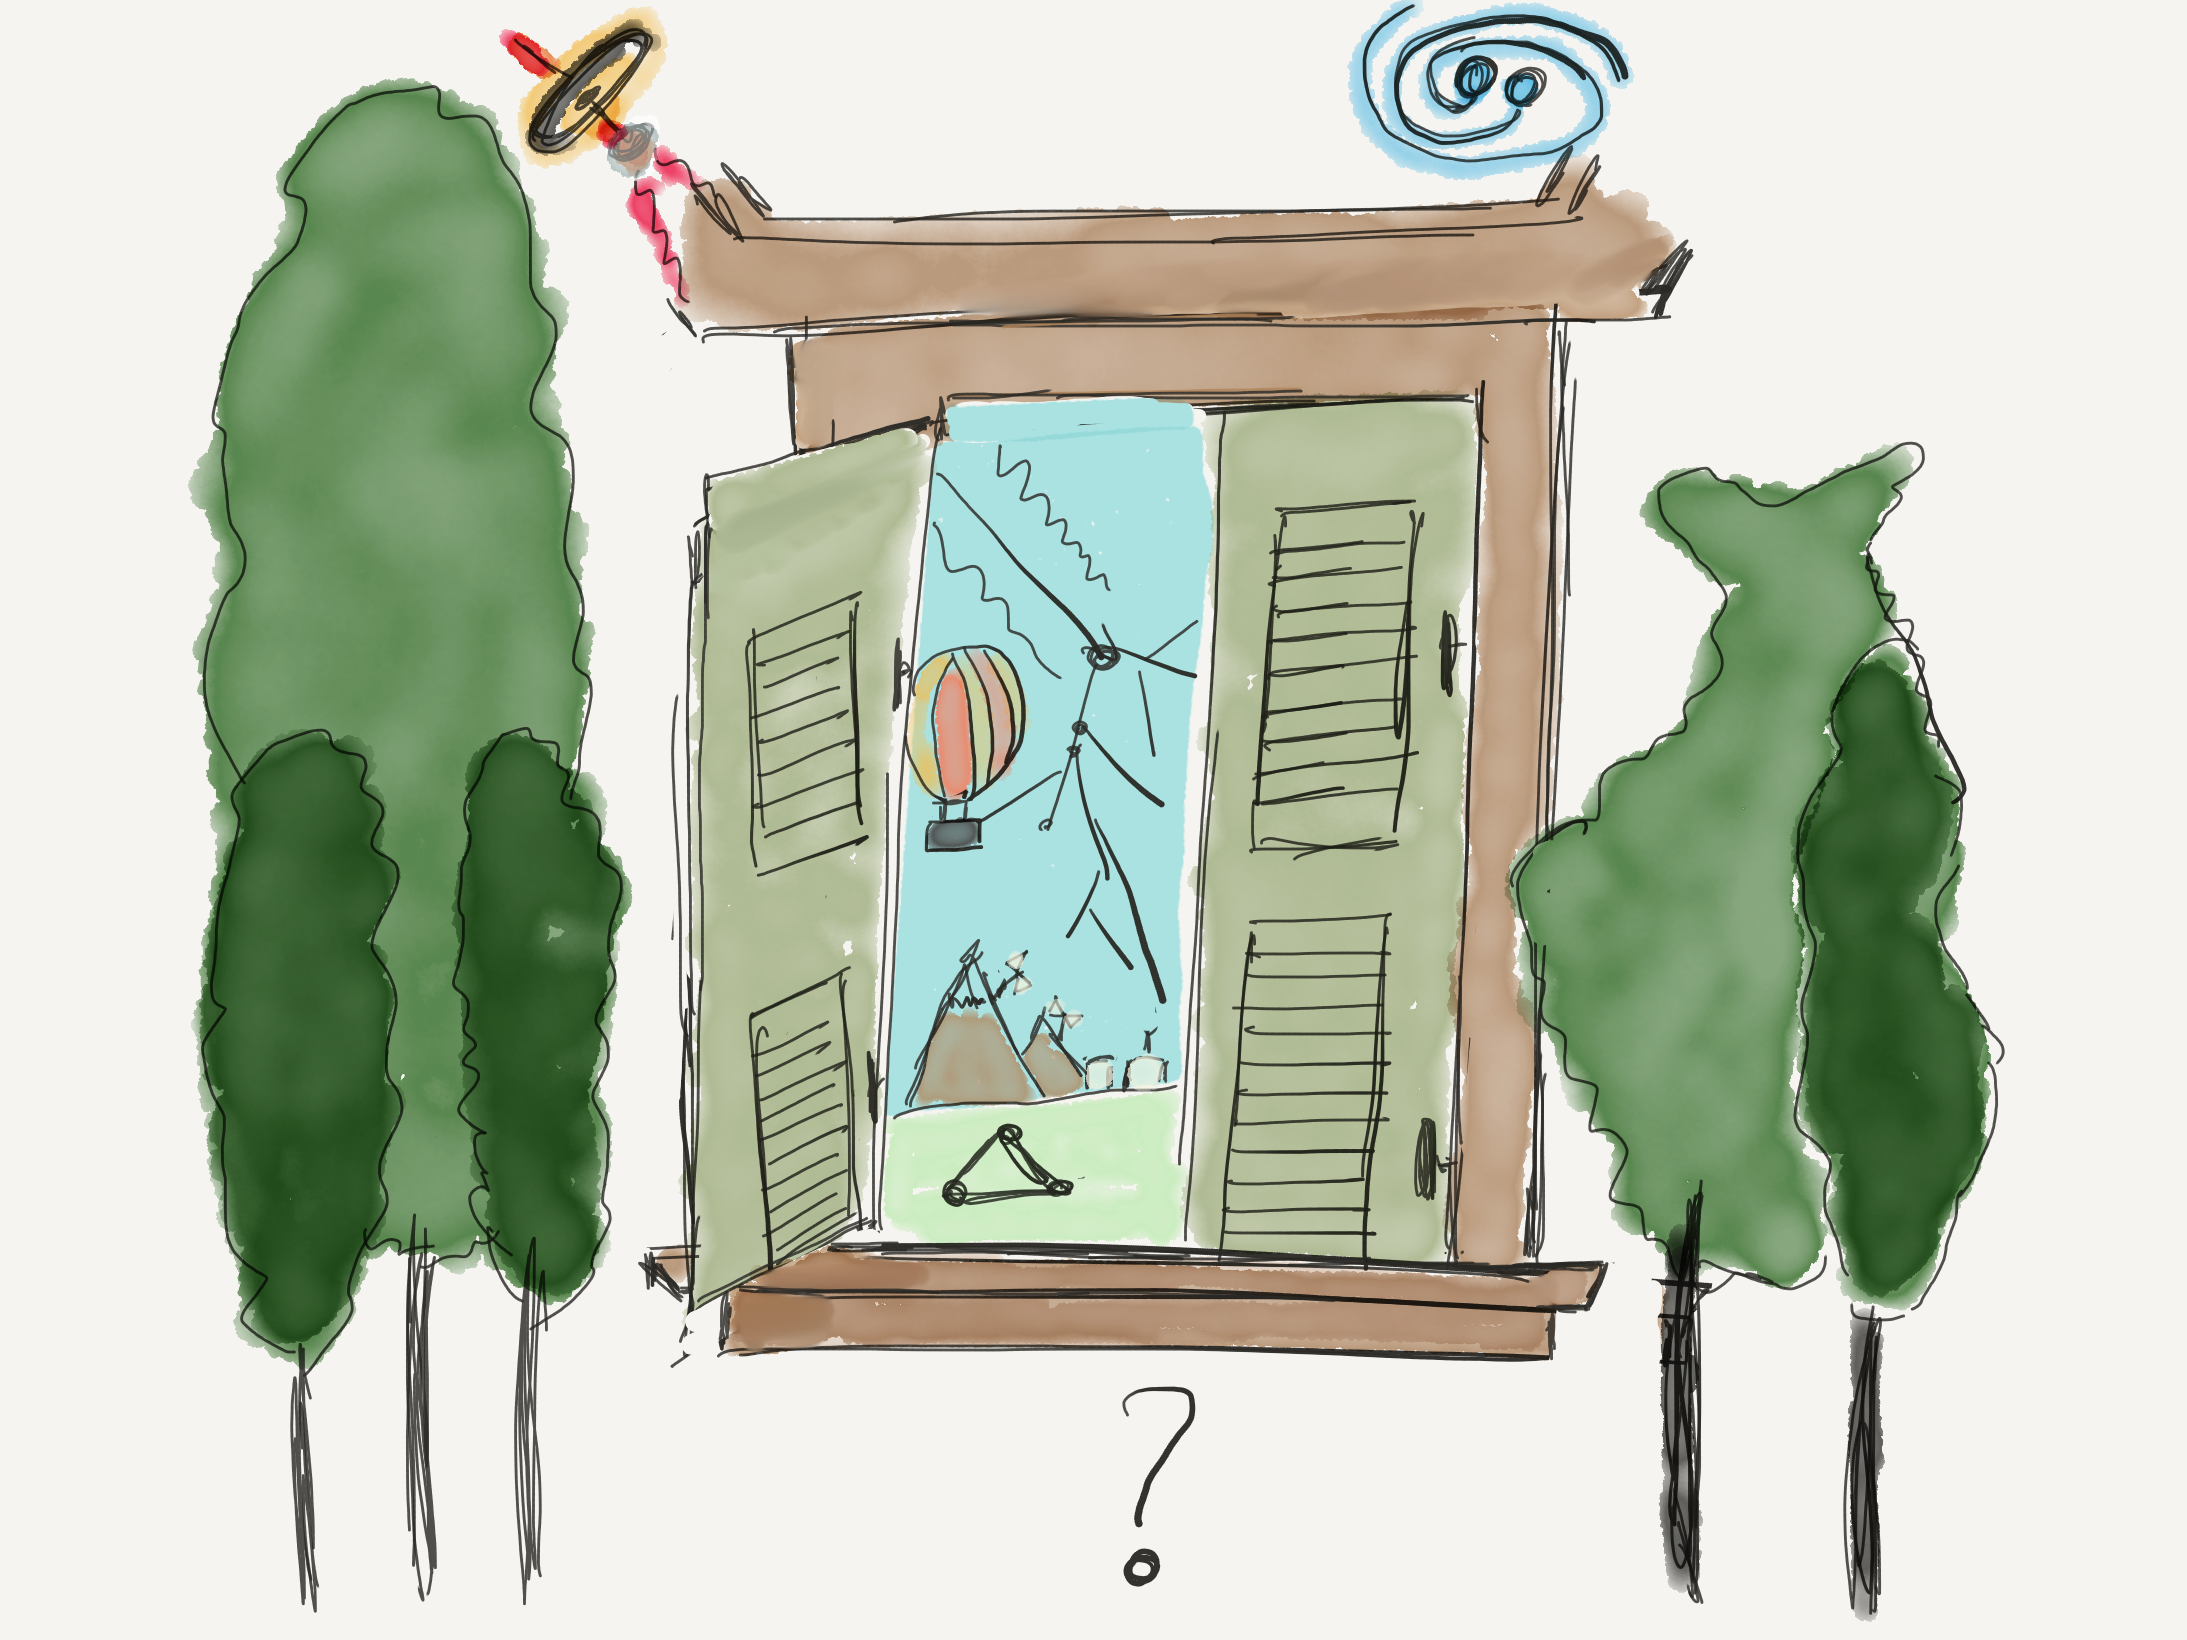
\includegraphics[width=13cm]{thesis_figures/What?.png}
\caption{Window to the inner workings of the Universe is only half opened. (better caption?)}
\label{fig:intro}
\end{figure}
The need to understand how something works or why something is? is ingrained in every human. While attempting to find answers for these questions one either answers them conclusively or finds oneself asking additional questions stemming from the original. One such question which bothered physicists at the beginning of the 20th century and eventually led to the field of \textit{astro-particle physics} was of so-called "atmosphere electricity" or ionization of air. After the pioneering discoveries by Theodor Wulf~\cite{article_Wulf} and Victor Hess~\cite{Hess:1912srp} who found the increase of this ionization rate with altitude and theorized the origin of this radiation to be not earth but something above our atmosphere, the name \textit{cosmic rays} was coined by Robert Millikan who believed these rays were originating from primary photons. This hypothesis was rejected by the measurements done by Jacob Clay~\cite{Clay:1927I,Clay:1928II} in 1927 who observed a latitude dependence of the intensity of cosmic rays concluding this to be a deflection of the primary cosmic-rays(CRs) by the geomagnetic field of the earth which indicated that these rays must be charged particles. After this came the efforts of B. Rossi~\cite{rossi1933eigenschaften}, German group~\cite{schmeiser1938harten} and P. Auger~\cite{RevModPhys.11.288} all independently discovering coincident signals in separated Geiger counters which they explained by the counters being struck by an extensive particle shower triggered by a primary cosmic ray. The phenomenon was named \textit{sciami} by Rossi, \textit{Luftshauer} by the German group and "Auger showers" by Auger and his collaborators. Auger went one step further by further estimating the primary energy of the cosmic ray via his superior setup giving rise to some questions about CRs which are yet unanswered, how are they created and where are they coming from. One of the known sources which is the Sun is too close to explain some other high energy CRs constantly hitting the Earth's atmosphere. Since then the field has only expanded with numerous experiments set up to characterize these cosmic rays. 

The biggest of these experiments which looks for ultra-high energy cosmic rays(UHECRs) exists in 3000 km$^2$ patch of Argentinian pampa just outside Malargue called the Pierre Auger Observatory~\cite{Auger:2015}. It uses a combination of 1660 Water Cherenkov tanks which form the Surface Detector of the observatory and observe the air shower particles arriving at the ground along with Fluorescence Detectors/Telescopes which can look at the development of shower as it travels through the atmosphere. Built primarily to answer the question of the cut-off of the cosmic ray spectrum also known as Greisen–Zatsepin–Kuzmin limit(or GZK cut-off), the observatory has provided immense contributions not only in the field of CRs but also in the fields of Geophysics(elves)~\cite{Mussa_2022}, Dark matter(composition)~\cite{Abreu_2023} and multi-messenger physics(neutrino+photon searches)~\cite{Aab_2019_point,Auger_photons_2022}. Currently, the Surface detector is undergoing an upgrade which will add a scintillator and radio detector on top of the Water Cherenkov tanks further increasing the sensitivity of the Observatory especially to the composition of the cosmic rays.

The non-electrical neutrality of the incoming CRs provides one of the biggest hindrance for finding their sources. This means that CRs do not travel in straight lines from their sources and are affected by the magnetic fields and can also interact with the matter along the way~\cite{bister2024largescaleanisotropyfluxdemagnification, ALLARD201233}. Combined with the fact that the possible sources are light years away from us, without knowing the magnetic fields of the Universe it is very hard to detect the sources of CRs. Ultra High Energy Neutrinos (UHE$\nu_s$) can help in this challenging search for the sources of CRs~\cite{UHEcorrelation_2016}. Being electrically neutral and having a very low interaction cross-section these particles can travel large distances unaffected by the intervening matter and magnetic fields. Several scenarios which are discussed later in section.~\ref{subsubsec:CRmessengers} describe how the UHE$\nu_s$ can be produced by cosmic-rays and can tell us about their sources. Moreover, UHE$\nu_s$ are also interesting as they can also help constrain or explain different production and propagation scenarios for various sources helping us see known astrophysical and cosmogenic objects in a new way. The success of IceCube Neutrino Observatory, a neutrino observatory located in the South Pole,  in detecting the first astrophysical neutrinos and observations of the first steady source NGC 1068~\cite{Icecube_2022} and transient source~\cite{Icecube_txs} have reinvigorated the astro-particle field. The Pierre Auger Observatory has also contributed to the search for UHE$\nu_s$ by trying to detect the Extensive Air SHowers (EASs) that can be induced by them. With its stellar sensitivity at high energy, searches at Pierre Auger Observatory have provided some of the strictest upper limits on the diffuse flux of UHE neutrinos~\cite{Aab_2019_diffuse}. This has already led to constrains on various hypothesized models explaining cosmogenic neutrino production.

The last decade with the successes of LIGO/VIRGO~\cite{PhysRevLett.116.061102} in measuring the first Gravitational waves and IceCube in detecting the first astrophysical neutrinos has also rekindled a field which displays the true spirit of harmony in science and is called multi-messenger astronomy. The aim of the field is to establish a network that can coalesce all the information available through various messengers via which we can see the Universe and maximise the resources and experiments available at Earth. This also allows us to understand the sources better since the observation or non-observation of different messengers can help constrain the mechanisms behind their functioning. The beginning of this field can be traced back to the observation of the first cosmic rays in conjunction with solar flares further cementing the important role Pierre Auger Observatory can play for this field. One of the most important success stories of this field is the August 2017 detection of the neutron star collision~\cite{Abbott_2017} first by the LIGO/VIRGO detector since the Gravitational waves are the fastest messengers and then 1.7s later by the Fermi Gamma ray space telescope and INTEGRAL. 11 hours later already alerted by these two experiments the optical counterpart was detected by multiple telescopes like Las Campanas Observatory and the Hubble Space Telescope. The event was also further seen in Ultraviolet(Neil Gehrels Swift Observatory), X-ray(Chandra X-ray Observatory) and radio(Karl G. Jansky Very Large Array). The non observation of neutrinos by both the IceCube and the Pierre Auger Observatory helped reach the important conclusion about the orientation of the jets which is hypothesized to be off-axis i.e. not pointing directly towards the Earth. Since neutrinos and Gravitational waves are the fastest of the messengers to reach the Earth, alerts issued by IceCube and LIGO/VIRGO are regularly used to follow up the events with other experiments. Subsequent observations of the blazar TXS 0506+056~\cite{TXS_Multi_2018} with IceCube, FERMI-LAT and MAGIC and the observations of neutrinos from the plane of the Milky Way galaxy~\cite{Galactic_plane_nu_2023} have helped establish the continued importance of multi-messenger astronomy.

In this thesis performance of one of the upgrades of the Pierre Auger Observatory done in 2013 is evaluated in the context of neutrino search. This upgrade consisted of introducing new triggers called Time over Threshold deconvulated(ToTd) and Multiple of Positive Steps(MoPS) to reduce the muonic background and effectively decrease the energy threshold for the array. Such triggers can be particularly important in the context of neutrino searches between $60^\circ$-$75^\circ$ since they help in getting a better signal background separation. The effect of these triggers for both the search of a diffused neutrino flux and point like sources of neutrinos is investigated. The thesis also focuses on maximising the previously done neutrino searches in the zenith region $60^\circ$-$75^\circ$ by investigating and updating the analysis presented in~\cite{Aab_2019_diffuse},~\cite{gap_note_2013}.

The thesis is structured as follows, The next chapter~\ref{chap:crnNu} gives the theoretical background for UHE cosmic rays and UHE neutrinos and other important messengers in regard to the Pierre Auger Observatory. It also aims to discuss the various theoretical scenarios involved in their production and propagation. The chapter also aims to summarize the important recent results for these messengers and the various interesting open questions for them. The next chapter~\ref{chap:EAS} describes the phenomenon of Extensive Air showers which is used to indirectly detect both the cosmic rays and neutrinos at the Pierre Auger Observatory. To continue with understanding the detection in a more experimental context the next chapter~\ref{chap:setup} gives a detailed description of the Pierre Auger Observatory. The objective of the chapter is to try to give an exhaustive description of all the tools at the Pierre Auger Observatory necessary to detect neutrinos with a particular focus on the Surface Detector which is of primary concern for the analysis presented in this thesis. A small section is also dedicated to the recently completed AugerPrime upgrade and the exciting potential it offers especially for multi-messenger searches. 

The second part of the thesis is dedicated to the neutrino search in the zenith angular region $60^\circ$-$75^\circ$ (Down-going low, DG$\mathrm{_{low}}$). This part begins with the chapter~\ref{chap:DGL} that gives a description of the neutrino search in the angular range $60^\circ$-$75^\circ$ which is also the primary focus region for this thesis. The chapter is dedicated to provide a complete description of the choices made for the analysis with the proper reasoning. It reports the areas of potential improvements and also communicates the observed improvements to the neutrino search with the new triggers. A new ~\textit{blind} search is performed to look for neutrinos in the data recorded at the Pierre Auger Observatory. The results are summarised at the end of this chapter and due to the non-observance of any neutrino like events, the corresponding limits to the neutrino flux are presented. The Observatory can also detect showers in zenith angle range $75^\circ$-$90^\circ$ (Down-going high, DG$\mathrm{_{high}}$) and up-going showers in the zenith angular region $90^\circ$-$95^\circ$ (Earth-skimming, ES)with the Surface Detector and $90^\circ$-$180^\circ$ (???) with the Fluorescence Detector, but these searches are not performed in this thesis and only their final results are included for comparison and to provide a holistic feel for the neutrino search at Pierre Auger Observatory.

The last part of this thesis presents an example of a neutrino follow-up analysis for point-like sources in chapter~\ref{chap:follow-up}. Due to the non-observance of any neutrinos in the data at the Pierre Auger Observatory an upper limit set by this analysis is also provided for interesting point source neutrino candidates. All the important results are then finally summarised in chapter~\ref{chap:conc} and a short outlook of the future directions for the analysis and the neutrino search at the Pierre Auger Observatory is put forward. The dissertation is completed by three appendices. The first describing the independent work done to compare the various hadronic interaction models for neutrino simulations and the second contains a technical overview of the changes made to implement the $75^\circ$-$90^\circ$ neutrino search within Offline, the software framework of the Pierre Auger Observatory. 

%%% Local Variables:
%%% mode: latex
%%% TeX-master: "mythesis"
%%% End:

% !TEX root = mythesis.tex

%==============================================================================
\chapter{Dark Photon $A'$}
\label{sec:darkp}
%==============================================================================
This section describes the theory and motivation for a new U(1) gauge boson that couples to the SM via kinetic mixing with the photon. The first indication of the existence of such a light boson was arrived at as an attempt to explain the astrophysical observations especially from PAMELA and WMAP/PLANCK. The explanation for the observed results was dark matter annihilation into $e^+e^-$. The PAMELA results required a large cross-section into leptons and a low cross-section into hadrons for the theorized particle. Taking this observation and building a model~\cite{Arkani_Hamed_2009} for this hypothesized particle already helped negate a few SM candidates such as Z, W and Higgs bosons (all (three) have low cross-section into leptons) and thermal WIMP (low cross-section at small lorentz boosts)~\cite{Arkani_Hamed_2009}, which is a competing dark matter prospect. Occurrence of a light vector boson that annihilates to leptons might explain these observations. Such a boson $A'$ was added to the SM in the simplest way by introducing a new spontaneously broken U(1) gauge field which couples via kinetic mixing with the ordinary photon, first discussed in \cite{HOLDOM1986196,GALISON1984279}. The Lagrangian is modified in the following way:
\begin{equation}\label{eq:Lagrangian}
  {\cal L} =  L_{SM} - \frac{1}{4} F'_{\mu\nu}F^{\mu\nu} + \frac{\epsilon}{2} F'_{\mu\nu}F^{\mu\nu} + \frac{m^2_{A'}}{2} A'_{\mu}A^{\mu} + i \overline{\chi} \gamma^{\mu} \partial_{\mu} \chi - m_{\chi} \overline{\chi} \chi - e_D \overline{\chi} \gamma^{\mu} A'_{\mu} \chi
\end{equation}
here $A'_{\mu}$ is the field associated with the dark photon, $\frac{\epsilon}{2} F'_{\mu\nu}F^{\mu\nu}$ is the kinetic mixing term between the dark photon and SM photon with $\epsilon$ describing the mixing strength. $\chi$ is treated as a placeholder for dark matter fermions which couple to $A'$ via the coupling constant $e_D$ also known as the dark portal coupling constant, $m_{A'}$ and $m_{\chi}$ are the masses of the $A'$ and the dark matter fermion respectively. The $A'$ can aquire its mass via the Higgs~\cite{PhysRevLett.13.508} or the Stueckelberg~\cite{Kors:2005uz} mechanism.

The mixing between the SM photon and $A'$ offers a possible channel for its production such as the high energy electron scattering off a nuclei $e^-Z\rightarrow e^- Z A'$. The production cross-section of $A'$ for this reaction was calculated using improved Weizsäker-Williams (IWW) approximation and the exact tree-level (ETL) calculations by Liu et al. \cite{Liu:2017htz} and Gninenko et al. \cite{Gninenko:2017yus}. This calculation is extremely important since it gives us a theoretical prediction for the number of $A's$ that could be produced for this channel and is also useful for the implementation of a MC simulation for the reaction.

\begin{figure}[t!]
\centering
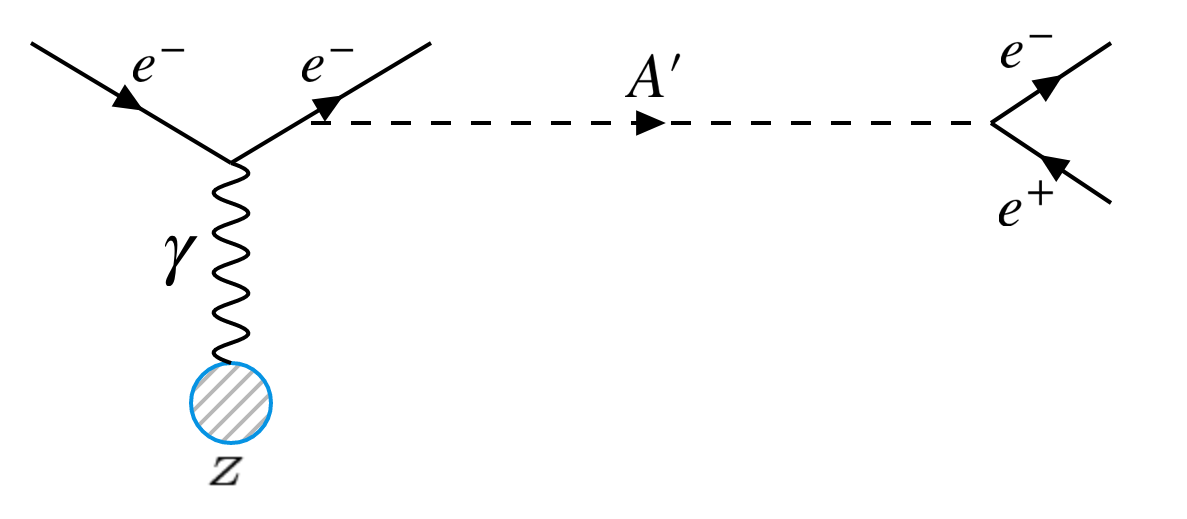
\includegraphics[width=14.5cm]{thesis_figures/VISIBLE.png}
\caption{Visible mode }
\label{fig:Visible_feynman}
\end{figure}

\begin{figure}[t!]
\centering
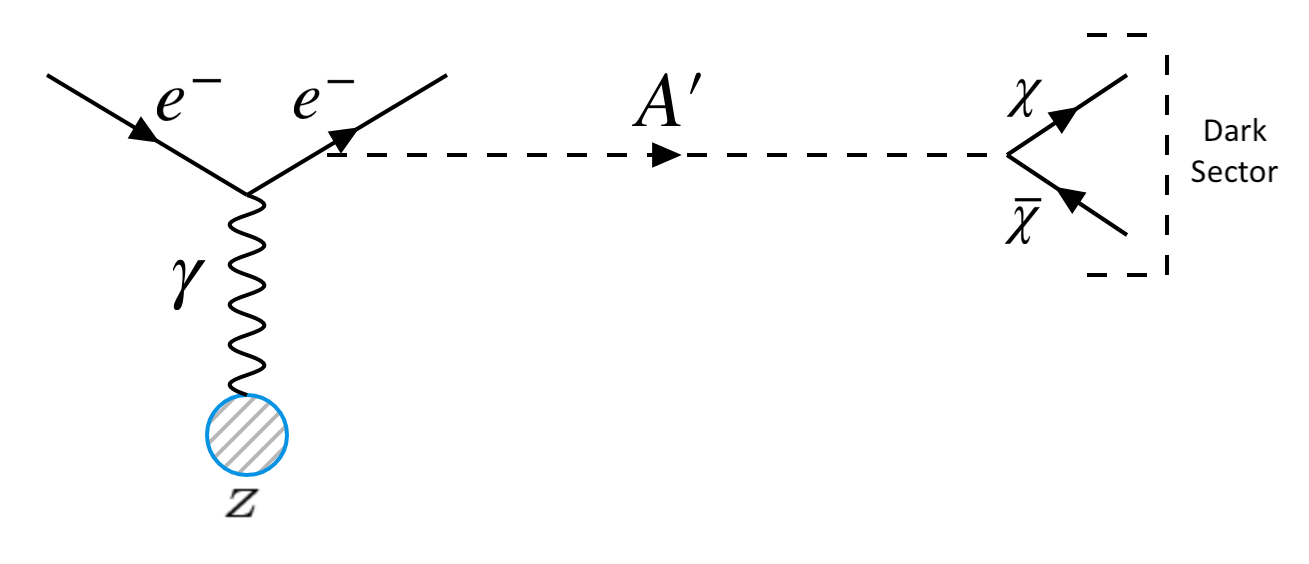
\includegraphics[width=15cm]{thesis_figures/INVISIBLE.png}
\caption{Invisible mode }
\label{fig:Invisible_feynman}
\end{figure}
Clearly from eq.(\ref{eq:Lagrangian}) there are two possibilities for the detection of $A'$. It can be either observed via its decay to SM particles which is called the \textit{visible mode} (fig.(\ref{fig:Visible_feynman})) or via its decay to light DM particles known as the \textit{invisible mode} (fig.(\ref{fig:Invisible_feynman})). In the visible mode we assume that $A'$ is one of the lightest states in the dark sector, then it is fair to believe that it would mainly decay to SM leptons. Such an interaction is described by the Lagrangian ${\cal L}_{int} = \epsilon e A'_{\mu} J^{\mu}_{em}$ where $J^{\mu}_{em}$ is the electromagnetic current and $e$ is the electromagnetic coupling. Such a decay would assume the $A'$ to have a sub-GeV mass and $\epsilon \ll 1 $. It also allows for an opportunity to set up an experiment for this particular mode since we will directly observe an excess of leptons in the final state. On the other hand for the invisible mode we assume that $A'$ is not the lightest state and there exists some other state $\chi$ with a lower mass, such that $A'\rightarrow \chi \overline{\chi}$ is a possibility. Such an event can also be probed with a so called missing energy experiment where the produced $A'$ or $\chi$ carries away some of the energy and is not detected.

The production and detection mechanisms discussed offer us the basic ingredients needed to set up an experiment for the detection of $A'$. One of the simpler layouts for such an experiment is an electron beam dump experiment. NA64 falls in this category, the setup of which is discussed in the next chapter.
\begin{figure}[t!]
\centering
  \begin{minipage}[t]{.45\textwidth}
    \centering
    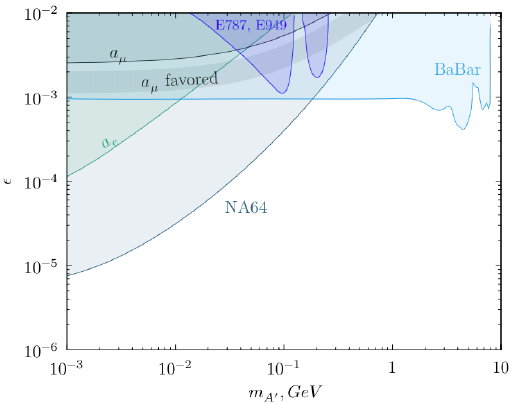
\includegraphics[width=\textwidth]{thesis_figures/exclusion_invisible.png}
    \caption{Current limits for invisible mode for 90\% C.L. exclusion region in the ($m_{A'},\epsilon$) plane ~\cite{2019EPJWC.21206005K}.}
    \label{fig:exclusion_invisible}
  \end{minipage}
  \hfill
  \begin{minipage}[t]{.45\textwidth}
    \centering
    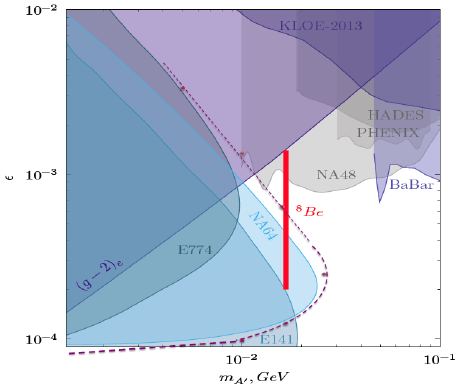
\includegraphics[width=\linewidth]{thesis_figures/exclusion_visible_latest.png}
    \caption{Current limits for invisible mode for 90\% C.L. exclusion region in the ($m_{A'},\epsilon$) plane. The blue plane is with 2017 data and the dotted line is with 2017+2018 data for NA64. The red line is the region that might explain the X17 boson~\cite{2019EPJWC.21206005K}.}
    \label{fig:exclusion_visible}
  \end{minipage}
\end{figure}


%%% Local Variables:
%%% mode: latex
%%% TeX-master: "mythesis"
%%% End:

% !TEX root = mythesis.tex

%==============================================================================
\chapter{NA64 Experimental Setup}
\label{sec:setup}
%==============================================================================
\begin{figure}[h!]
\centering
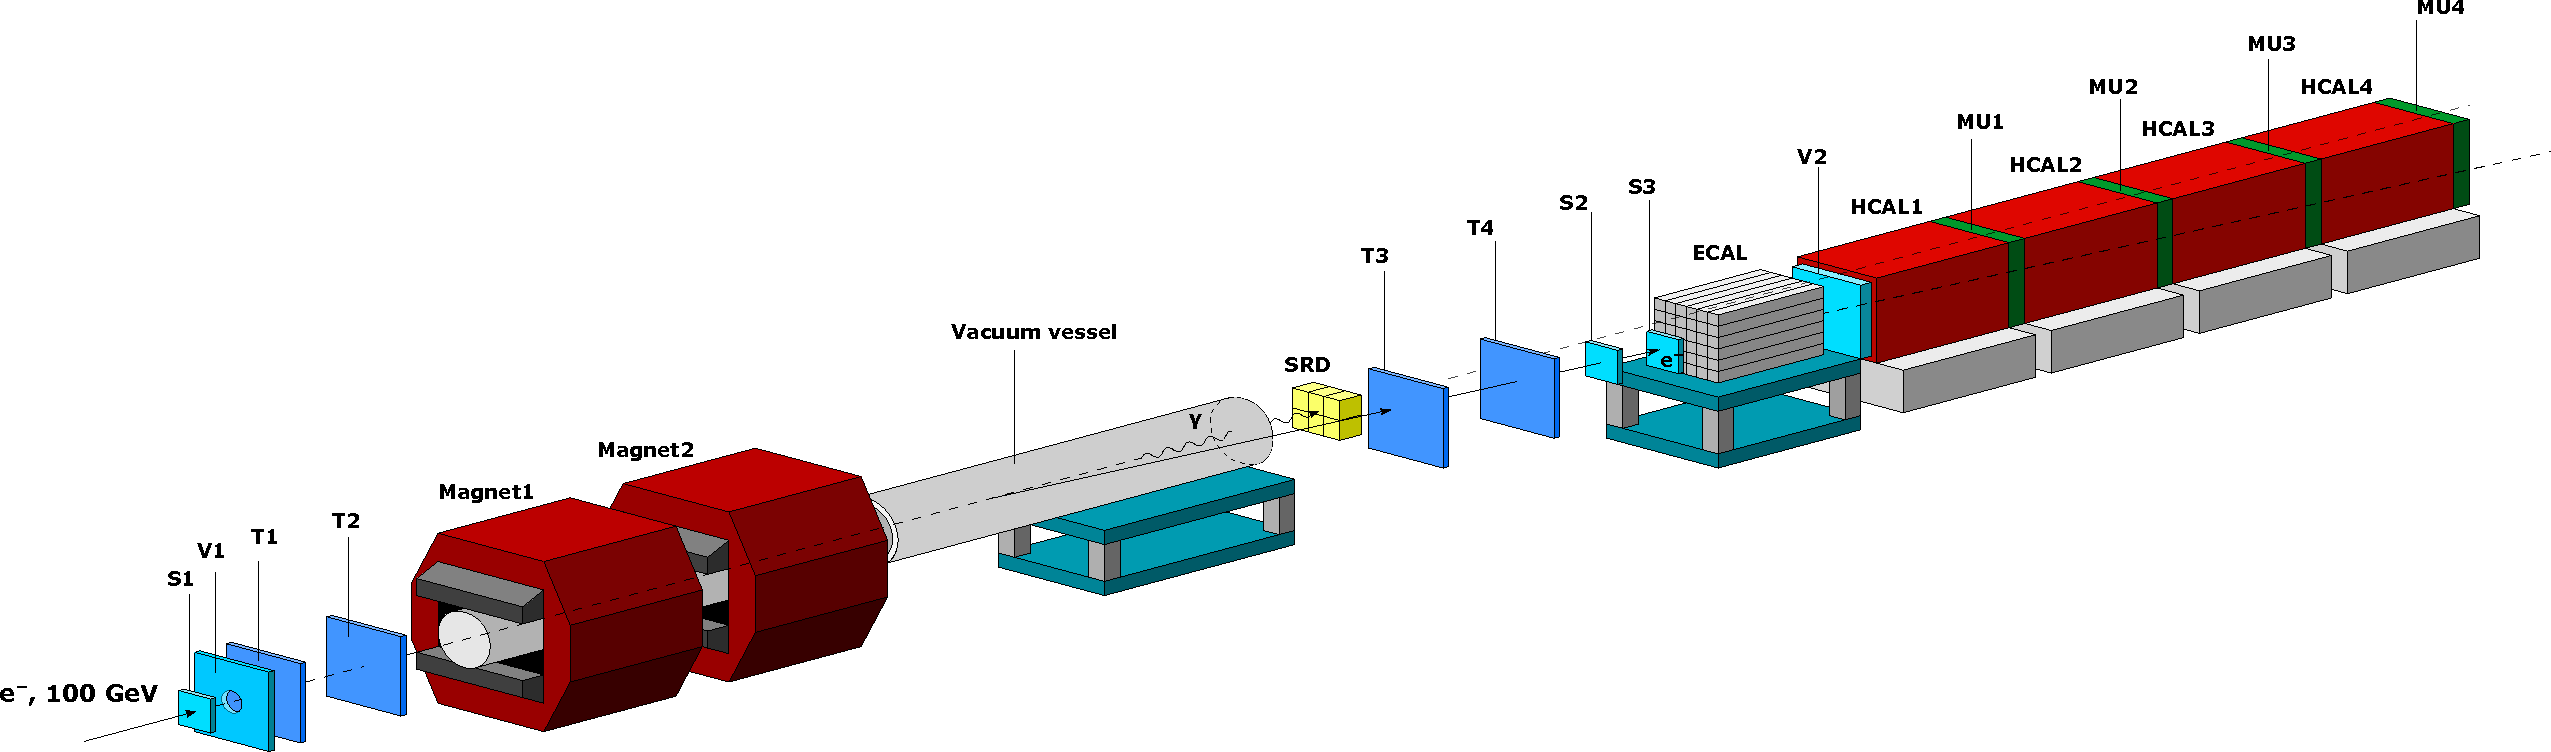
\includegraphics[width=\textwidth]{thesis_figures/Invisible_3d_setup.png}
\caption{Invisible mode setup~\cite{Banerjee:2016tad}}
\label{fig:Invisible_mode_setup}
\end{figure}

NA64 is a beam dump fixed-target experiment located at the H4 beam line of the Super Proton Synchrotron (SPS) at CERN. The objective of the detector is to look for rare dark matter candidates, primarily Dark Photons $A'$. $A'$ is supposed to be emitted via a process similar to bremsstrahlung $e^-Z\rightarrow e^- Z A'$. The experiment is not a permanent fixture and has been in operation since March, 2016. Since it's approval the setup has taken data a total of four times which included a two week test run in 2016 and four weeks of data taking each in 2016, 2017 and 2018. Each year the setup has slightly varied to account for different beam energies and expected background.

The SPS provides a primary proton beam of $400~\mathrm{GeV/c}$ with $\simeq 10^{12}$ protons per spill which is then converted to electrons by incidence on a beryllium target. The $e^-$ beam is in the momentum range $50-150~\mathrm{GeV/c}$ with a maximal intensity $\simeq 10^{7}$ per SPS spill of 4.8s. The provided high-energy $e^-$ beam with the large luminosity was needed since the $A'$ couples very weakly to the SM. The beam is then characterized by passing it through scintillators (S1-S3),veto ($V_1$), two dipole magnets with an integral magnetic field of $\simeq 7~\mathrm{Tm}$ and trackers (MM-section(\ref{sec:MM}), GEM-section(\ref{sec:GEM}) contained in tracking stations (T1-T4) which measure the $e^-$ beam momenta to a 1\% precision~\cite{article_beam_purity}. Additionally the combination of magnets followed by a 15m long vacuum vessel and a PbSc synchrotron radiation detector (SRD) acted as a filter to reject low energy electrons and hadrons that might be present in the beam and would contribute to the overall background. They were separated by putting a cut on the amount of synchrotron radiation energy deposited by the respective particle~\cite{Gninenko:2013rka}. The beam is then allowed to hit the electromagnetic calorimeter (ECAL) which acts as an active target. The ECAL consisted of 6x6 Shashlik-type modules each with 40 radiation lengths ($\mathrm{X_0}$) of which the initial 4$\mathrm{X_0}$ is employed as a separate preshower(PS) detector. The ECAL had a resolution of $\delta E_{ECAL}/E_{ECAL} \simeq 0.1 \sqrt{E_{ECAL}[\text{GeV}]}$~\cite{Banerjee:2016tad}.
The combined information achieved by studying the shower and the SRD signal helped in suppressing the hadron contamination in the beam to a remaining fraction of $ \lesssim 10^{-6}$~\cite{Depero:2017mrr}. A combination of Veto($V_2$) and hadronic calorimeter(HCAL) is situated downstream of the ECAL. They serve as a veto against muons, neutrals like high energy photons or hadrons produced in the target ECAL. The HCAL consisted of four modules ($\text{HCAL}_{1-4}$) separated by muon counters ($MU_{1-4}$) and were slightly shifted along the beam with each module consisting of 3x3 cells adding up to a total of $\simeq$30 nuclear interaction length ($\lambda_{int}$). The HCAL had a resolution of $\delta E_{HCAL}/E_{HCAL} \simeq 0.6 \sqrt{E_{HCAL}[\text{GeV}]}$~\cite{Banerjee:2016tad}.

\begin{figure}[t!]
\centering
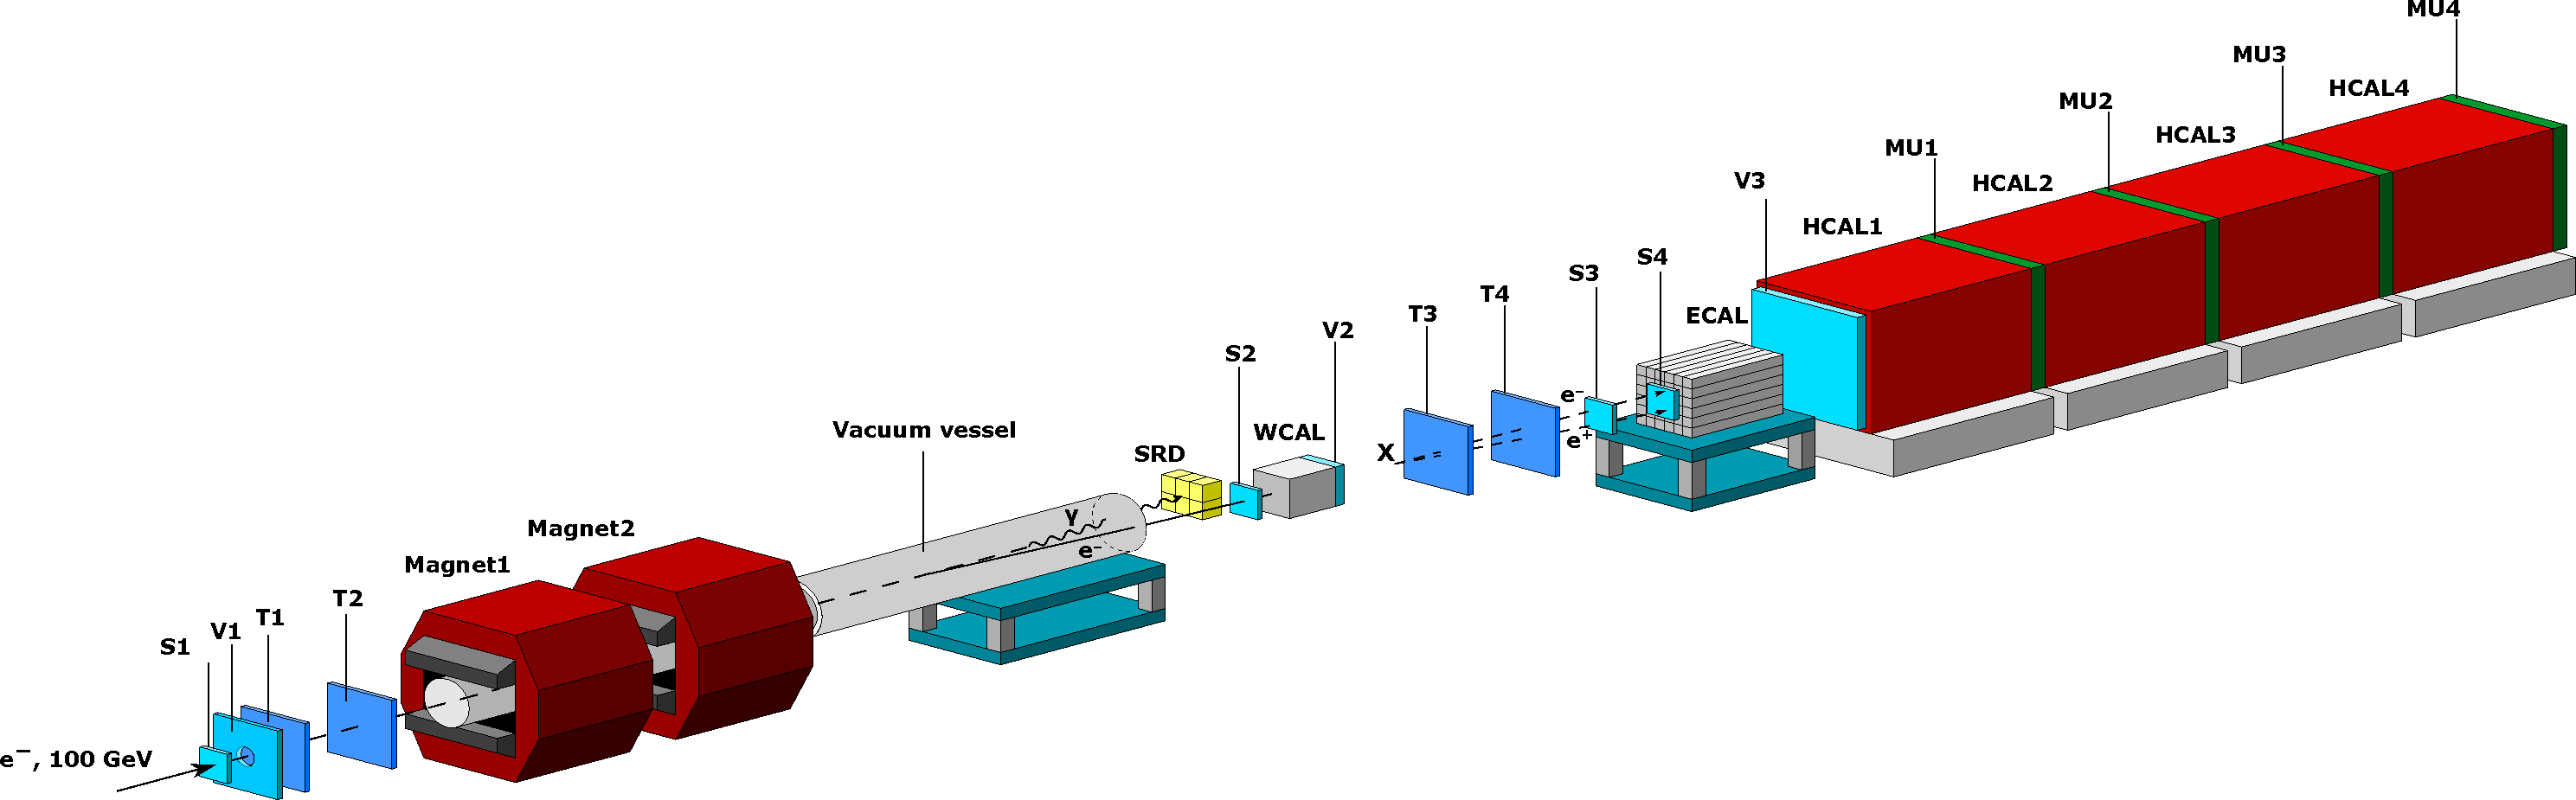
\includegraphics[width=\textwidth]{thesis_figures/Visible_3d_setup.png}
\caption{Visible mode setup 2017~\cite{Banerjee_2018}}
\label{fig:Visible_mode_setup}
\end{figure}

\begin{figure}[t!]
\centering
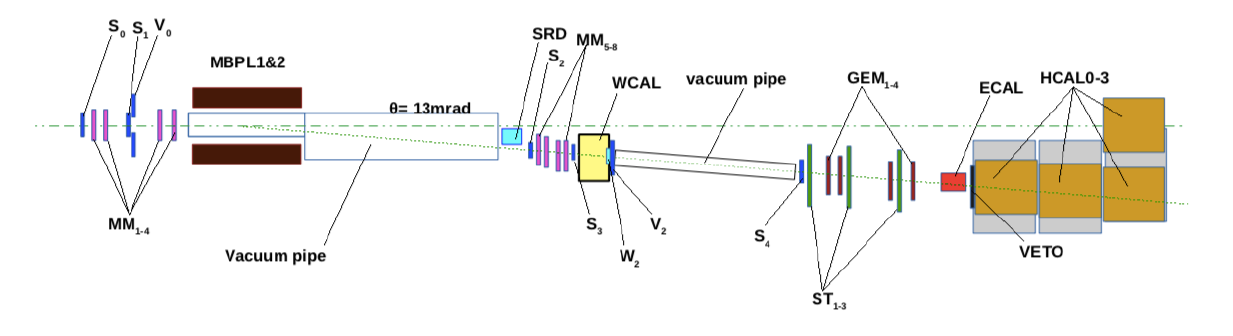
\includegraphics[width=\textwidth]{thesis_figures/visible_mode_newest.png}
\caption{Visible mode setup 2018-top view~\cite{Gninenko:2677228}}
\label{fig:Visible_mode_setup_side}
\end{figure}

The above setup works well for the \textit{invisible mode}($10^{-4} \lesssim \epsilon \lesssim 10^{-3}$, $m_{A'} \lesssim 1 \text{GeV}$) but requires modification for the search of $A'(X)$ in the \textit{visible mode}($10^{-4} \lesssim \epsilon \lesssim 10^{-3}$, $m_{A'} \lesssim 100 \text{MeV}$). To search for the visible decays a short tungsten calorimeter (WCAL) and a veto ($V_2$) were added right after the vacuum pipe and before the second set of tracking detectors (fig.(\ref{fig:Visible_mode_setup})). The size of the WCAL was selected so that the leakage of particles is small and the sensitivity to short lifetimes is maximized. The distance between the WCAL and the ECAL for the visible mode searches was slightly varied(2.5m->5.6m) between 2017 and 2018 which allowed for the installation of a 3.1m long vacuum tube to create better spacing between the ECAL and WCAL for a better angular resolution to increase the sensitivity to X17 bosons~\cite{Banerjee_2018}. A WCAL catcher was also installed in 2018 to prevent any leakage. Additionally the beam momentum was increased from 100GeV to 150 GeV in 2018 and one of the tracking station consisting of two MicroMegas (MM) was also shifted upstream of the WCAL. Counter ($W_2$) and straw detectors ($\text{ST}_{1-3}$) were also tested during the 2018 beam period(fig.(\ref{fig:Visible_mode_setup_side})). Both \textit{invisible} and \textit{visible} mode setups were also used to look for rare SM events that involve a photon decaying to a dimuon pair via bremsstrahlung $e^-Z\rightarrow e^-Z\gamma;\gamma\rightarrow \mu^{+} \mu^{-} $. Comparing these rare events, which were obtained from real data, to our Monte Carlo(MC) simulated sample helped in estimating the validity and efficiency of our MC simulation~\cite{Gninenko:2677228}.

In summary, NA64 tries to estimate and tag the beam $e^-s$ using a combination of trackers, SRD and ECAL/WCAL, uses the said ECAL/WCAL as an active target and then collects the residue of the interaction in the downstream HCAL/ECAL+HCAL. It also utilizes the hard bremsstrahlung photon to dimuon conversion as a measuring stick for the reliability of the MC simulations. The reactions of interest were attempted to be observed with a combination of hardware and software triggers depending on the expected signature of the decay mode for $A'$.

\textbf{Invisible Mode:}
$A'\rightarrow \chi \overline{\chi}$ signature:
\begin{flalign*}
  Beam(p\simeq 100~\text{GeV}),\\
  E_{ECAL+PS}(< 100~\text{GeV}),\\
  V_2(< E^{th}_{V}\simeq 1~\text{MIP}),\\
  E_{HCAL}(< E^{th}_{HCAL}\simeq 1~\text{GeV}).
\end{flalign*}

\textbf{Visible Mode:}
$A'\rightarrow e^+ e^-$ signature:
\begin{flalign*}
  Beam(p\simeq 150~\text{GeV}), \\
  E_{WCAL}(< 150~\text{GeV}), \\
  E_{WCAL+ECAL+PS}(\simeq 150~\text{GeV}), \\
  V_2(> E^{th}_{V}\simeq 1~\text{MIP}), \\
  V_3(< E^{th}_{V}), \\
  E_{HCAL}(< E^{th}_{HCAL}\simeq 1~\text{GeV}).
\end{flalign*}







%%% Local Variables:
%%% mode: latex
%%% TeX-master: "mythesis"
%%% End:

% !TEX root = mythesis.tex

%==============================================================================
\chapter{Tracking}
\label{sec:tracking}
%==============================================================================
This chapter gives a brief summary of the hardware and the software used to implement tracking for NA64. It begins with a description of the detectors used to track the incoming beam at NA64. Further it describes the algorithm implemented to fit tracks to the information received from the detectors. It ends with a brief description of the software where the said algorithm is implemented.

\section{Detectors}
NA64 uses two varieties of Micro-Pattern Gas Detectors (MPGD) to track the beam particles and estimate their momentum. MPGDs offer a high rate capability along with a spatial resolution O($\mathrm{\mu m}$), both of which are required for NA64. They work on the basic principle that charged particles moving through a medium interact with it in different ways losing some energy in the process. The interaction in case of MPGDs is a direct Coulomb interaction with the atoms present in the detector medium leading to their ionization. The two varieties are the following:
\subsection{MicroMegas}
\label{sec:MM}
MICRO-MEsh GAseous Structure (Micromegas) were invented in 1992 by Georges Charpak and Ioannis Giomataris~\cite{CHARPAK200226} as an alternative to Multi-Wire Proportional Chamber (MWPC)~\cite{Sauli:1977mt} to counter its space resolution and rate limitations.

In a MicroMegas (MM) detector a metallic mesh is introduced between the anode and cathode. The mesh itself is supplied with a high voltage effectively separating the detector volume into two regions. When a charge particle traverses the detector region above the mesh it will ionize the atoms present in the medium. The electrons produced in this process drift towards the mesh where they encounter a high electric field reaching enough energy to create an avalanche. The electrons from the avalanche induce a signal on the readout electrodes while the ions are collected by the mesh. A schematic of the detector is shown in fig.(\ref{fig:Micromegas_na64}) and a more detailed description of the process can be found in \cite{CHARPAK200226}.

The NA64 Micromegas are resistive Micromegas where the usual single readout layer is replaced with a layer of resistive strips (R) followed by additional readout layers below. They were developed at the CERN EP-DT-EF workshop~\cite{Banerjee:2017mdu}. The readout is made up of two layers of 320 strips(X and Y) perpendicular to each other, both rotated by an angle of $45^{\circ}$ with respect to the global reference system and are therefore called U and V throughout the thesis. The strips which are parallel to the resistive strips have a lower capacitive coupling compared to the ones which are perpendicular leading to a slightly worse positional resolution in one plane. The detector was measured to have a gain of $\approx 2 \times  10^4 $ at an amplification voltage of 540 V~\cite{Banerjee:2017mdu}.

\begin{figure}[t!]
\centering
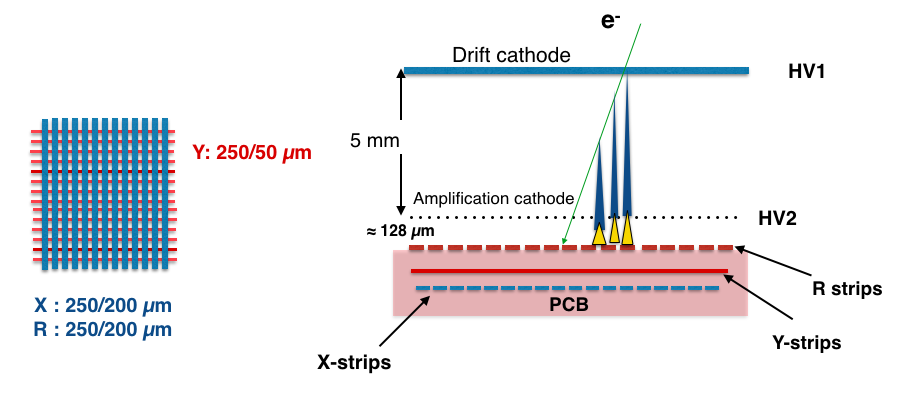
\includegraphics[width=\textwidth]{thesis_figures/NA64_MM.png}
\caption{Left: Strip dimensions of the modules, Right:NA64 Micromega's working principle~\cite{Banerjee:2017mdu}}
\label{fig:Micromegas_na64}
\end{figure}

\subsection{Gas Electron Multiplier}
\label{sec:GEM}
 Gas Electron Multiplier (GEM) was invented by F.Sauli at CERN in 1997. They are cheaper and easier to manufacture compared to other tracking detectors and offer a flexible geometry thus can be used in different shapes and sizes. They have versatile applications as they can be used both as a standalone detector and as readout elements of a Time Projection Chamber (TPC).

 A standard GEM detector consists of a single or multiple layers of  GEM foils inserted between drift and charge collection electrodes. Each foil is made up of polymer coated with a thin metal layer on both sides. The foil is punched with a high density of holes. The holes are etched on both sides of the foil forming a double-conical structure as shown in fig.(\ref{fig:GEM_field}), other kind of hole shapes are also possible. When a differential voltage is applied to the electrodes the holes develop field lines as shown. Electrons drifting through the holes will follow the field lines gaining enough energy to ionize the filled gas leading to an avalanche. Electrons from the avalanche are then collected by the readout  electrode. A more detailed description of the process can be found in~\cite{SAULI20162}.

 The NA64 GEMs were developed at the Technical University Munich (TUM)~\cite{Baust:2008} and resemble the ones developed for COMPASS~\cite{Ketzer:2001dt}. They consist of three stacked GEM foils followed by a stripped readout. The readout consists of two layers perpendicular to each other (X and Y) which are aligned the same as the global reference system. The detector is filled with a mixture of $\mathrm{Ar/CO_2}$ in a ratio of 70/30. The gain of the detector was measured to be $\approx 8 \times 10^4 $ at detector voltage of 4050V~\cite{hosgen:2017}.

 \begin{figure}[t!]
 \centering
   \begin{minipage}[t]{.45\textwidth}
     \centering
     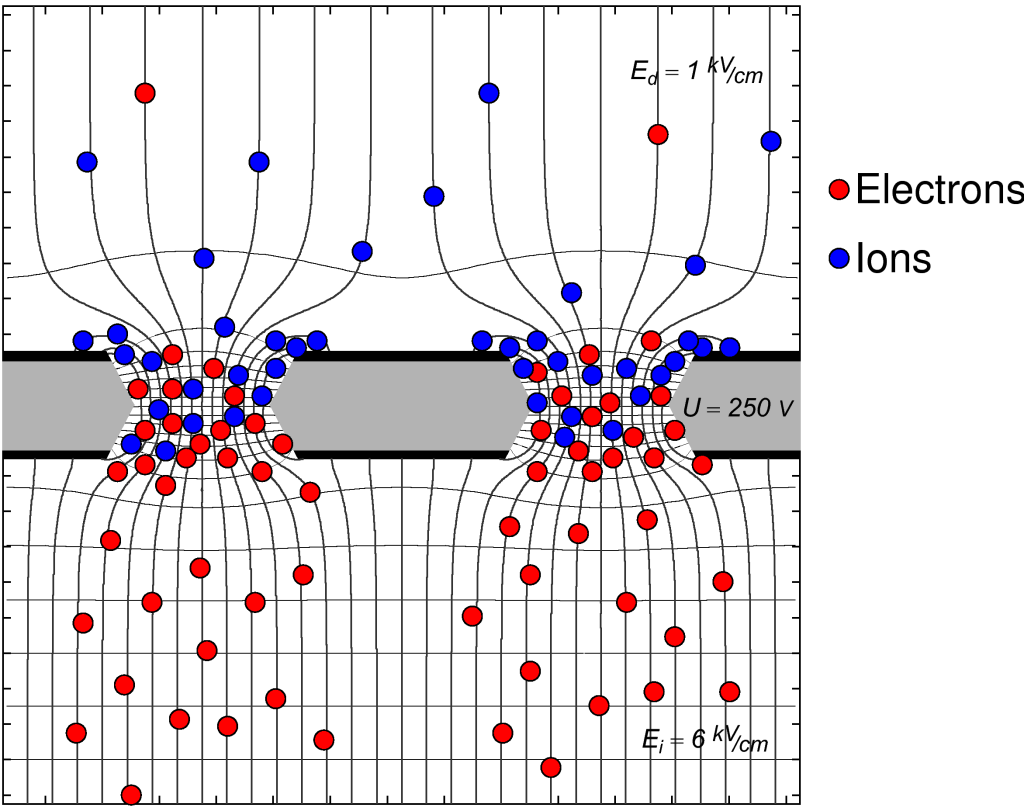
\includegraphics[width=\linewidth]{thesis_figures/GEM_field.png}

     \caption{A sketch of GEM field lines~\cite{GEM_field}.}
     \label{fig:GEM_field}
   \end{minipage}
   \hfill
   \begin{minipage}[t]{.45\textwidth}
     \centering
     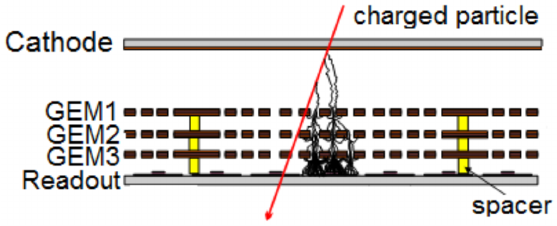
\includegraphics[width=\linewidth]{thesis_figures/GEM_process.png}
     \caption{Schematic of a triple GEM detector along with the working principle~\cite{article_GEM_pic}}
     \label{fig:Triple_GEM}
   \end{minipage}
 \end{figure}

\section{Track-Reconstruction Algorithm}
This section describes the methods used to fit a track to the output obtained from the tracking detectors and to extract momentum information of the beam from this data. For a simple setup this can be done by fitting a straight line through the hits on the detectors for the regions before and after the magnet obtaining the angle between the two lines to estimate the momentum. This method is described under Linear Regression. For a more complex tracking system and to simulate a more realistic picture for the beam and better alignment for the detectors, the Kalman filter algorithm is used to fit the tracks.

\subsection{Linear Regression}
\label{sec:Linear_Regression}
Linear regression for track fitting involves fitting a straight line to the data points, hits in our case with the condition that the total error is minimized. The total uncertainty is calculated as a sum of squares of individual measurement errors. Since the final result is dependent on minimizing the sum of the squares this approach to linear regression is known as least-squares approach. A simple mathematical description of the method is given below.

The equation of a straight line is given by $y=mx + c$, where $m$ is the slope of the line and $c$ is the intercept on the $y$ axis in a Cartesian coordinate system. The final goal is to obtain a good estimate for the two parameters $m$ and $c$. To obtain this estimate the square of error needs to be minimized. The error is the difference between the actual measurement $(x_i,y_i)$ and the prediction from our model, the equation of straight line. This error is also known as the residual and is defined as $r_i = y_i - m x_i - c $ for an $i^{th}$ measurement. Suppose that $n$ hits are measured then to obtain an estimate for $m$ and $c$ we need to minimize $\sum_{i=1}^n r_i^2$. The minimized estimates have the following values:
\begin{equation}
      \text{min}(m) = \frac{\sum_{i=1}^n x_i y-i - 1/n \sum_{i=1}^n x_i \sum_{i=1}^n y-i}{\sum_{i=1}^n x_i^2 - 1/n ()\sum_{i=1}^n x_i)^2}  = \frac{\bar{xy} - \bar{x}\bar{y}}{\bar{x^2-\bar{x}^2}}
\end{equation}
\begin{equation}
      \text{min}(c) = \bar{y} - \text{min}(m) \bar{x}
\end{equation}

A more detailed mathematical description can be found in \cite{Linear_regression}. The quality of the fit can be evaluated by calculating the reduced chi-square $\chi^2_{red}=\frac{\chi^2}{ndf.}=\frac{1}{ndf.}\sum_i \frac{(r_i)^2}{\sigma^2}$ where $\sigma$ is the resolution of each detector which might not be equal and ndf. are the number of degrees of freedom available for the fit.

Linear regression can also be used for NA64 to fit for the bending due to the magnets by replacing the model function from the equation of the straight line to some polynomial function. Such a method is called polynomial regression~\cite{STIGLER1974431}.

\begin{figure}[t!]
\centering
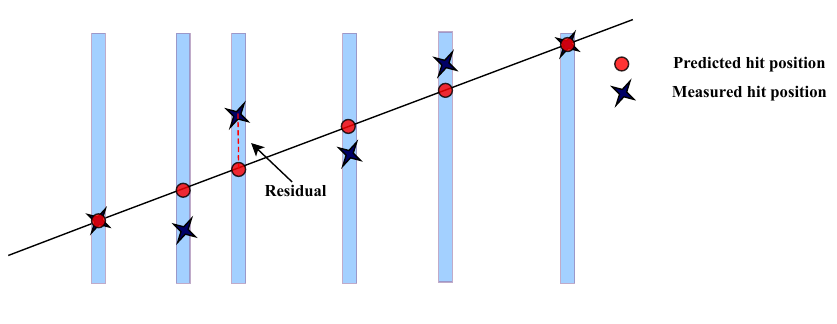
\includegraphics[width=\textwidth]{thesis_figures/linear_reg_new.png}
\caption{Linear regression pictorially. }
\label{fig:linear_regression}
\end{figure}

\subsection{Kalman Filter}
Kalman filter is an estimation technique originally developed to predict rocket trajectories. In particle-physics it is often used as an iterative least-square estimation procedure for track fitting. Following is a brief description of the algorithm for track fitting which closely follows~\cite{Fruhwirth:1987fm,Astier:412374}.

Let's assume for a given track model $x_k$ be the value of the "ideal measurement" at the intersection point between the track and the detector at some point k. This is also called the state vector of the system and in an iterative procedure where the value at location $k$ is obtained from a previous location $k-1$ can be written as :
\begin{equation}
  x_k = f_k(x_{k-1}) + w_k
\end{equation}
where \textbf{f} is the track model propagator function and in this form propogates from detector $k-1$ to $k$ and $w_k$ is a random vector representing the noise between the two detector positions such as multiple scattering perhaps.

\begin{figure}[t!]
\centering
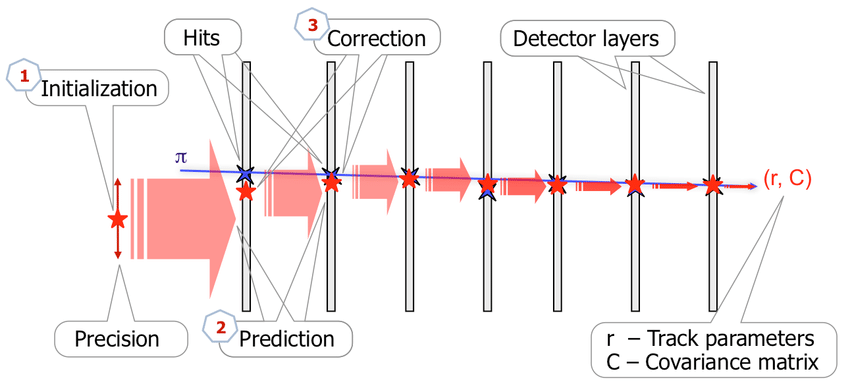
\includegraphics[width=\textwidth]{thesis_figures/KALMAN.png}
\caption{Pictorial representation of the working principle of a Kalman filter ~\cite{article_KALMAN}.}
\label{fig:Kalman_filter}
\end{figure}

Now, the state vector is not a quantity that is measured directly by the detector. If we assume that $m_k$ is the value of the measurement by detector k then it can be given as :
\begin{equation}
  m_k = h_k(x_k) + \epsilon_k
\end{equation}
$h_k(x_k)$ is the function of the state vector measured at the detector which in our case will be a position measurement by our tracking detector. $\epsilon_k$ represents a measurement noise which for an ideal measurement will be zero. We assume that both $w_k$ and $\epsilon_k$ are independent random variables and have a mean value of zero.
For a linearized system,
\begin{equation}
  f_k(x_{k-1}) = F_k x_{k-1}
\end{equation}
\begin{equation}
  h_k(x_{k-1}) = H_k x_k
\end{equation}
There are three key operations that need to be performed for the Kalman filter procedure. These are ordered and described with respect to time specifically to handle multiple scattering in a proper manner.
\begin{description}
  \item $\bullet$~\textbf{Filtering} is estimating the "present" state vector taking into account all the present and "past" measurements. Filtering from $m_1$ to $m_k$ includes filtering $m_1$ to $m_{k-1}$, then propagating from $m_{k-1}$ to $m_k$ and including $m_k$.
  \item $\bullet$~\textbf{Prediction} is estimating the state vector at a "future" time.
  \item $\bullet$~\textbf{Smoothing} is estimating the state vector at any point based on all the measurements.
\end{description}

The basic process can be described as follows. If we have an estimate at position $x_{k-1}$ then it can be extrapolated to position $x_k$ by using the system equation. The estimate at $x_k$ is calculated as a weighted mean between the prediction from the system equation and the measurement from the measurement equation $m_k$. This estimate is passed to all the previous estimates in parallel by using the smoother which is running in a backward direction. Also if there is no process noise $w_k$ then smoothing is equivalent to back extrapolation.

\textbf{System equation:}
\begin{equation}
  x_k = F_k x_{k-1} + w_{k}
\end{equation}
\begin{equation}
  E{w_k} = 0,  \mathrm{Cov[w_k]} = Q_k (1\leq k \leq N)
\end{equation}
\textbf{Measurement Equation:}
\begin{equation}
  m_k = H_k x_{k} + \epsilon_{k}
\end{equation}
\begin{equation}
  E{\epsilon_k} = 0,  \mathrm{Cov[\epsilon_k]} = V_k = G_k^{-1} (1\leq k \leq N)
\end{equation}

As an example here are the different processes for one update step:

\begin{description}
\item $-$ Prediction - Extrapolation of the state vector
      \begin{equation}
        x_k^{k-1} = F_k x_{k-1}
      \end{equation}
      Extrapolation of covariance matrix :
      \begin{equation}
        C_k^{k-1} = F_k C_{k-1} F_k^T + Q_k
      \end{equation}

\item $-$ Filtering - Update of state vector
       \begin{equation}
         x_k = C_k [ \, (C^{k-1}_k)^{-1} x_k^{k-1} + H_k^T G_k m_k ] \,
       \end{equation}
       Update of covariance matrix :
       \begin{equation}
         C_k = [ \, (C^{k-1}_k)^{-1} + H_k^T G_k H_k ]^{-1} \,
       \end{equation}

\item $-$ Smoothing - Smoothed state vector
      \begin{equation}
        x_k^{N} = x_k + A_k(x_{k+1}^N - x_{k+1}^k)
      \end{equation}
      where $A_k$ is called the smoother gain matrix given by: $A_k = C_k F_{k+1} ^T (C_{k+1}^k)^{-1}$

\end{description}
Other information such as residuals $r_k$, covariance matrix of residuals $R_k$ and $\chi^2$ for each step are also calculated and incorporated during the fitting process. A global $\chi^2_{trk}$ is a sum of all chi-squares from filtering. After the Kalman fitting we have three fits for the parameters at a particular hit at position $k$: a track fit for the part upstream i.e  using measurements from 1 till $k$, a backward track fit for the part downstream using measurements from $N$ till $k$ and a fit for the whole track.

The Kalman filter can also be applied for a non-linear system such as in the presence of a magnetic field, by the replacement of the track propagator $f_k$ with the first two terms of of its Taylor series expansion. With this change the procedure is known as extended Kalman filter. This procedure is implemented in the track fitting libraries in CORAL. The computational time of the filter is directly proportional to the number of detector and does not depend much on the total amount of hits in an individual detector. A potential drawback of the algorithm is that it needs initial starting parameters for the state vector and its covariance matrix. This is usually solved by either fitting a small number of measurements with linear regression and then feeding it to the algorithm or by starting with an arbitrary value for the state vector and covariance matrix.

\section{CORAL and PHAST}
CORAL is the reconstruction and analysis software used at COmmon Muon and Proton Apparatus for Structure and Spectroscopy (COMPASS). PHysics Analysis Software Tool (PHAST) was developed later to separate the analysis from reconstruction and works on the output obtained from CORAL. CORAL was envisioned as a modular program that consists of standard libraries for different processes such as track reconstruction and alignment, that are controlled using external option files. Different detectors can be added externally in a detectors table (detectors.dat) which is fed to CORAL along with the measured data file. The libraries of the detectors that are used at the NA64 experiment such as the Micromegas, which are a little different compared to the standard COMPASS ones, were also added to CORAL~\cite{hosgen:2017}.

The track reconstruction process in CORAL works in the following way. The detectors are divided into separate zones either depending on the magnets or depending on obstruction by a detector such as a calorimeter both of which is true especially in the visible mode for NA64. Zones before and after the magnets are fitted with straight line segments depending on the measurements. The line segments in each zone are then bridged together through the magnets which is sped up with an external Dico file. A Dico file consists of all the possible trajectories pre-calculated, for a particular geometry or setup. The last step in the track reconstruction process is a Kalman filter taking the initial information from the previous two steps and running over the entire track piece, combining the measurements into the final prediction. The momentum is determined according to the integrated magnetic field and the bending angle observed for the fitted track. The option file for track reconstruction for NA64 controls the input and output files for the whole process and also contains information about various noise cuts implemented for the detectors which are described in detail in \cite{hosgen:2017}.



%%% Local Variables:
%%% mode: latex
%%% TeX-master: "mythesis"
%%% End:

% !TEX root = mythesis.tex

%==============================================================================
\chapter{Alignment}
\label{sec:align}
%==============================================================================
Measuring charged particles precisely and efficiently is a crucial part of any particle physics experiment. This need is intensified more for NA64 since we need a very accurate estimate for the beam momentum and energy to look for missing energy events for the \textit{invisible mode}. NA64 also requires an accurate track reconstruction for the \textit{visible mode} to look for $e^+ e^-$ tracks that might originate from a possible $A'$. While the experiment was being installed a big emphasis was given to measure the outer boundaries of the detectors using lasers. Nonetheless this precision is insufficient when extrapolated to get an estimate for the inner part of the detector. Since the detectors are expected to have a micrometer precision, track based alignment will provide a better estimate for the actual detector positions and will help improving the errors in the final physics analysis. This chapter describes the program \textbf{Millepede} implemented for the track based alignment for NA64 and also reports the different types of alignment performed for the current setup. The results of alignment program are also compared to the standalone alignment method described in \cite{nabeel:2018}.

\section{Previously used method}
\label{sec:prev_used}
The previously used method~\cite{nabeel:2018} which was used for alignment in NA64 is a simple residual fit and shift. A short description of the steps involved in this procedure is as follows:
\begin{enumerate}
    \item The raw data which contains the hit information along with the detectors table is fed to CORAL for track reconstruction. Kalman filter is used for track reconstruction.
    \item The output from the reconstruction is obtained in form of a mini data storage (mdst) format which is analysed using PHAST.
    \item Residuals are calculated and fitted with a standard Gauss function to extract the peak for the residuals. An example for a specific plane is shown in fig.(\ref{fig:res_GEM4x}). This procedure is performed for each plane of the detector.
    \item The fitted peaks are the shifts for the detectors and for a good alignment should be centered to zero. These shifts are applied to the detectors table. For the next iteration the new updated detectors table is used as an input to CORAL.
    \item The number of iterations are selected by looking at the change in the reduced chi-square. This procedure is not automated at this point.
\end{enumerate}
Such a procedure has many limitations and can even lead to situations where there are simultaneous shifts in opposite directions. This procedure can only align for the X and Y planes of the detector and is not currently structured to include rotation of the planes of the detector. These problems are described in detail by V.Blobel in \cite{Blobel:2006yh}.

\begin{figure}[t!]
\centering
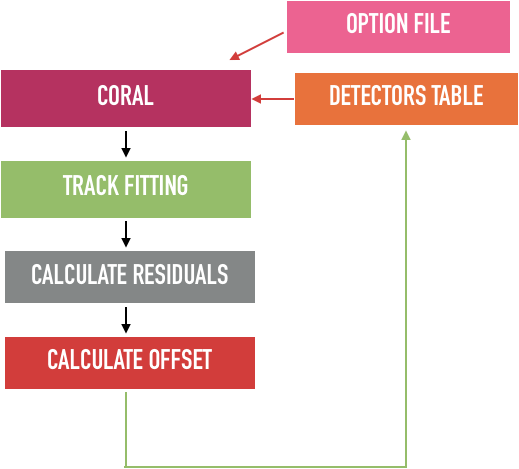
\includegraphics[width=0.65\textwidth]{thesis_figures/Previous_method.png}
\caption{Pictorial representation of the previously used method}
\label{fig:previously_used_flowchart}
\end{figure}

\begin{figure}[t!]
\centering
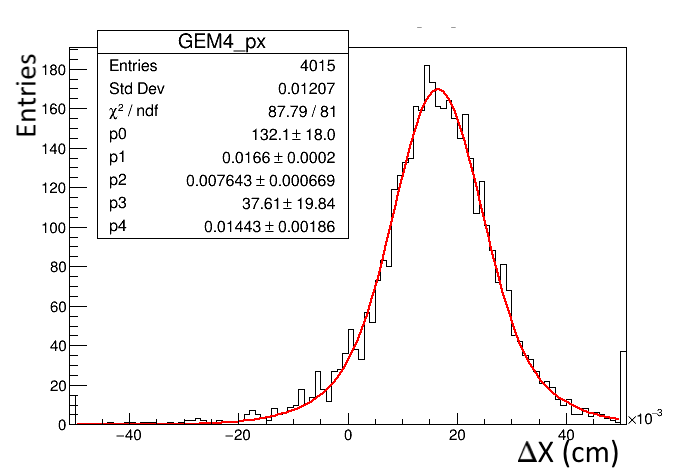
\includegraphics[width=0.65\textwidth]{thesis_figures/alignment/Residual_GEM4X.png}
\caption{Fitting of the residual for the X plane of GEM4}
\label{fig:res_GEM4x}
\end{figure}
%\FloatBarrier
\section{Millepede}
Millepede is an iterative alignment program that uses the linear least square method to fit and minimize all the relevant alignment parameters. The method and the initial implementation was developed by V. Blobel from the University of Hamburg and is maintained by  Deutsches Elektronen-Synchrotron (DESY) \cite{Millepede}. It is a smarter implementation of the previously used method that decreases the computation time while giving comparable results. The alignment parameters that Millepede tries to minimize can be seperated into two categories: \textit{global} and \textit{local}. Global parameters consist of sets of values that affect all data such as expected shifts for the detectors. On the other hand local parameters are values that are concerned with a single track such as slope, curvature etc. The previously used method ignores the global parameters and only aligns using individual tracks from measured events. If one of the detectors has a lot of noise for some reason the iterative residual based alignment may fail. This and many other reasons such as an inability to tangle correlated parameters while aligning makes the previously used method inferior compared to Millepede.

Following is the mathematical description of the Millepede algorithm which is closely adapted from \cite{Blobel:2002ax,Blusk:2007zza}.
Let the local parameters be denoted by $l_j$ where j is the  running index dependent on the complexity with which the track is described. For a general measurement the set of measurements at a detector plane k is given by
\begin{equation}
  y_k = l_1 \cdot \delta_{1k} + l_2 \cdot \delta_{2k} + ...l_n \cdot \delta_{nk} = \sum_{j=1}^n l_j \cdot \delta_{jk}
\end{equation}
where $\delta_j$ are some known constant factors. For example if the track measured at a detector, at position k, is a straight line track then: $y_k = l_1 \cdot 1 + l_2 \cdot S_k  $, where $l_1$ is the intercept and $l_2$ is the slope of the measured track. Here we assumed that the measurements are only dependent on local parameters. Similarly if we include global parameters $g_j$ then
\begin{equation}
  y = l_1 \cdot \delta_{1} + l_2 \cdot \delta_{2} + ...l_n \cdot \delta_{n} + g_1 \cdot h_{1} + g_2 \cdot h_{2} + ...g_n \cdot h_{u} = \sum_{j=1}^n l_j \cdot \delta_{j} + \sum_{i=1}^u g_i \cdot h_i .
\end{equation}
Linearising the above equation for a single point measured at location $x_i$ and track $k$ yields:
\begin{equation}
  y = f(x_i;\textbf{g},\textbf{l}) + \Bigg(  \frac{\partial f(x)}{\partial \textbf{g}_i} = d_i^{global} \Bigg)^T  \Delta\textbf{g} + \Bigg( \frac{\partial f(x)}{\partial \textbf{l}_i} = d_i^{local} \Bigg)^T  \Delta\textbf{l}_k
\end{equation}
with $f(x_i;\textbf{g},\textbf{l})$ being the mathematical model predicting the track and $\Delta\textbf{g}$ and $\Delta\textbf{l}$ are the corrections applied to global and local parameters after one iteration of a track fit.

The least square method requires us to solve the following matrix equation:
\begin{equation}
\begin{bmatrix}
    \sum_k C_k^{global} & \dots & H_k^{global-local} & \dots \\
    \vdots & \ddots & 0 & 0 \\
    (H_k^{global-local})^T & 0 & C_k^{local} & 0 \\
    \vdots & 0 & 0 & \ddots
\end{bmatrix}
\times
\begin{bmatrix}
    \Delta \textbf{g} \\
    \vdots  \\
    \Delta \textbf{l}_k \\
    \vdots
\end{bmatrix}
=
\begin{bmatrix}
    \sum_k b_k^{global}  \\
    \vdots  \\
    b_k^{local} \\
    \vdots
\end{bmatrix}
\end{equation}
here C is a symmetric matrix formulated as $C = \sum_{k=1}^m w_k d_k d_k^T $ with $w_k = 1/\sigma_k^2$ being the weight assigned to each measurement and $m$ being the total number of global parameters being fitted and $d_k$ being the derivative of the model with respect to the global parameter. A similar formulation is made for local parameters. $H_k$ is a matrix formulated in a similar way as to C and is defined as $H= \sum_k w_k d_k^{global} (d_k^{local})^T$. $b$ is the correction vector defined as $b = \sum_k w_k r_k d_k$ with $r_k$ being the residual as defined in sec.(\ref{sec:Linear_Regression}).

The Millepede algorithm implements a simultaneous fit for all tracks, including both local and global parameters. Since we only care about corrections to the global parameters the computation is sped up by focusing on $\Delta\textbf{g}$ calculation for each iterative step and solving the equation $\Delta\textbf{g} = (C^{global})^{-1} b^{global}$.

The step by step process of the Millepede minimization can be explained as follows:
\begin{enumerate}
    \item Fit the track using a fitter such as Kalman and extract the best values for local parameters.
    \item Collect derivatives $d_k$ for all local and global parameters that need to be minimized.
    \item Update the matrices $C^{global}$ and $b^{global}$ for each track by simple addition. An extra step is needed to update matrix $C:= C - HVH^T$ which indirectly includes the changes applied to the local parameters while updating the global parameters.
    \item Repeat the above steps for all the available tracks.
\end{enumerate}

After all the tracks have been computed and the relevant global matrices have been calculated the final equation $\Delta\textbf{g} = (C^{global})^{-1} b^{global}$ is solved. The inversion while calculating this equation is made even faster by partitioning the matrix into symmetric sub-matrices which is one of the special features of Millepede and is described in detail in \cite{Blobel:2002ax}.

The whole process of looping over all tracks and then computing the correction to the global parameters counts as one iteration of the Millepede algorithm. The selection for the number of iterations depends on the number of global parameters being used and the correlation between them if any.


\section{CORAL Implementation}
The Millepede program is included as a separate library "millepede.f"  in CORAL. The algorithm is written in FORTRAN and H.Pereira \cite{PereiraDaCosta:1204557} introduced an interface for the algorithm into CORAL. The options available for global parameters that can be minimized are positional(U) alignment, angular(T) alignment, pitch(P) alignment, alignment for the z position of the detector along the beam and many more which are not relevant for our tracking detectors.

\begin{figure}[t!]
\centering
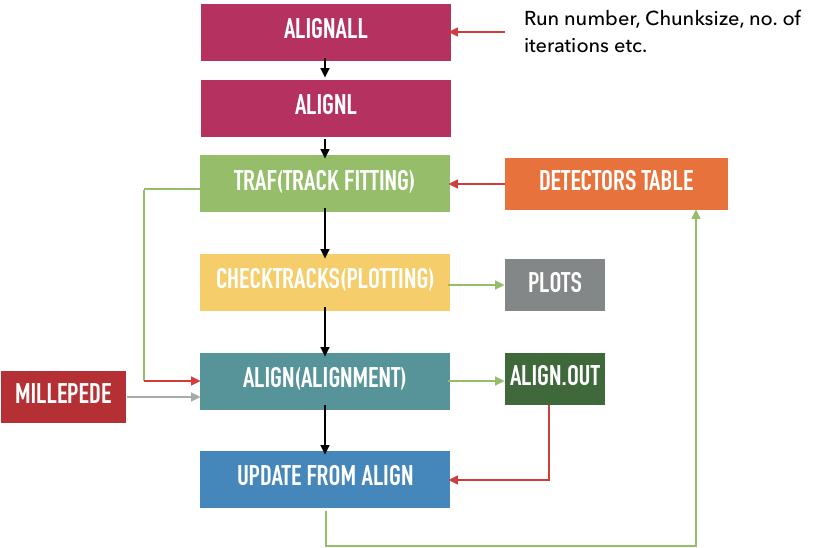
\includegraphics[width=\textwidth]{thesis_figures/Millepede_implementation.png}
\caption{ CORAL implementation of Millepede. The black lines signify the order of the steps while the green and red lines depict output and input respectively.}
\label{fig:millepede_implementation}
\end{figure}


The alignment method used in CORAL works on the standard Millepede condition which minimizes the sum of $\chi^2_{red}$ with respect to the local and global parameters. The method in CORAL is controlled using separate option files similar to the ones used in track fitting. The data flow for the whole alignment process is described in fig.(\ref{fig:millepede_implementation}).
\begin{description}
    \item $\Rightarrow$ "Alignall" and "Alignl" are bash scripts which are used in standard COMPASS alignment for staging the required data files for which the alignment needs to be performed. They also stage external files that CORAL needs such as the Dico file (faster bridging) for track fitting. The bash scripts are also involved in data management and in cleaning up of intermediate files produced during the alignment procedure. The bash scripts control the data flow and invoke different option files. the process begins by invoking the track fitting in CORAL which starts the alignment procedure. These scripts were adapted to work with NA64 and new options were introduced for the experiment.

    \item $\Rightarrow$ Track fitting uses the standard option file used for track reconstruction in NA64 with a few extra options. The most important option that is required to fill the root trees on which alignment works is "main do alignment". Other options such as whether to use the magnets and tracks having a non-zero momentum for alignment can also be set depending on the requirements. Both of these were used for the results mentioned in this thesis.

    \item $\Rightarrow$ Next the "checktracks" option is called. This option is used for plotting and checking the effect of each alignment step. It helps to achieve an immediate quality check and can be useful to spot errors in track reconstruction. It also gives basic information such as the alignment performance per iteration. For the first iteration step it gives the results of track reconstruction done on the setup where no software alignment was performed.

    \item $\Rightarrow$ Further, the "align" option is summoned. The "align" option is fed with the track reconstruction output from CORAL along with the detector positions. Moreover, the kind of global parameters that need to be minimized are specified at this stage. Other options such as aligning specific detectors, track selection cuts and inputting specific detector resolutions are also available. The Millepede minimization is invoked at this point. The "align" option gives an output with the required correction for each detector, for the particular global parameter that was aligned.

    \item $\Rightarrow$ Next the output from the "align" option is fed to "updateFromAlign". This tool applies the correction to the detectors table to create a new "detectors.dat" which is used for track fitting in the next iteration if multiple alignment iterations are performed.
\end{description}


\section{Results}
The alignment procedure was performed for the data collected during the 2017 invisible mode run for NA64. During this period, data taking and calibration were performed using a 100 GeV $e^-$ beam. The results of the alignment were tested by performing track fitting on the last obtained detectors table after all Millepede iterations were completed. The tracks used to obtain the quantifiable values for judging the results were chosen such that one hit from \textbf{each} detector plane contributed to the fitted track. In 2017 there were four Micromegas (MM1-MM4) upstream of the magnets and two Micromegas (MM5-MM6) and four GEMs (GEM1-GEM4) downstream of the magnets. The total number of detector planes available during the NA64 operational period were 19 since the Y plane of GEM3 was not operational. Since both the track fitting and alignment processes use detector resolution during minimization it is important to mention that for these results the resolution for GEMs was fixed at 50$\mu m$ and for Micromegas it was fixed to be 100$\mu m$. A random physics run with number 3211 was chosen to observe the results of the procedure. The results from this run were also compared to the ones obtained by the previously used procedure in \cite{nabeel:2018}. 500000 events per run were analyzed and CASTOR file system was used to access the data to study the process for a future run-by-run alignment application on the CERN computer cluster (lxplus). Different global parameters were minimized to study their individualized effects. The final conclusion about the quality of the alignment was drawn upon by looking at the reduced chi-square~ $\chi^2_{red}$ distribution and the distribution of residuals.

\subsection[Positional Alignment]%
{Positional Alignment} %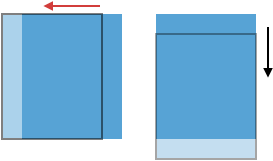
\includegraphics[width=20mm]{thesis_figures/positional.png}}

\begin{figure}[t!]
\centering
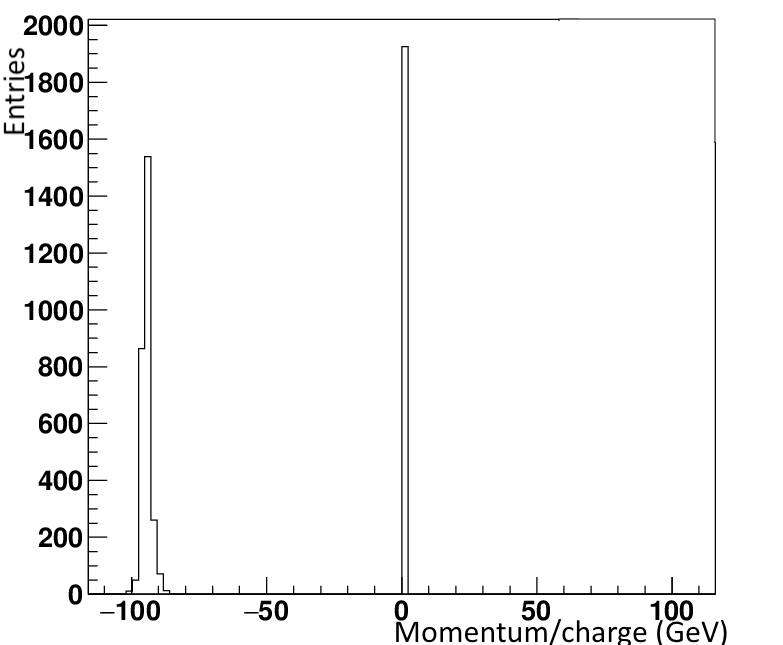
\includegraphics[width=0.65\textwidth]{thesis_figures/alignment/cop.png}
\caption{Charge over momentum distribution of all fitted tracks during alignment}
\label{fig:cop}
\end{figure}

The first global parameter which was aligned using the Millepede algorithm were the X and Y positions of the tracking detectors. In CORAL each readout plane of the detector is available to be aligned individually.
Positional(U) alignment refers to the alignment done to achieve an optimal (x,y) position for each detector plane. During the U alignment all detector planes were left free for movement in the (x,y) positions. However, other positional variables such as the angle with respect to the geometric reference system, z position and the pitch of the detectors were fixed. The tracks used for alignment were chosen to have $\chi^2_{red} < 100$ and a $-110 \text{GeV} <\text{p/charge}< -90 \text{GeV}$. The momentum over charge cut fig.(\ref{fig:cop}) made sure that only tracks that were bridged through the magnets were used for alignment. The results from the alignment are shown in figures (\ref{fig:GEM_residuals}), (\ref{fig:MX_residuals_1}) and (\ref{fig:MX_residuals_2}).

Ideally the residual distribution for a perfectly aligned detector should be centered around (0,0) which signifies that the measured hit position is accurately fitted during the track fitting procedure. As it can be seen from the figures, initially the residual distribution of almost all the detectors is displaced. Even though the observed displacement is small O(0.02cm), such a shift can hamper the positional resolution of the detectors which is expected to be of the O(~$\mu$m). This provides us with a visual proof that a software alignment is very much necessary. The final residual distribution after the Millepede alignment is much more uniform and is mostly centered around (0,0). The effect of the alignment is also measured by calculating the $\chi_{red}^2$ of all the selected tracks before and after alignment. We see in fig.(\ref{fig:red_chi2_1}) that the distribution shifts to a lower value which signifies that the alignment resulted in tracks with a lower $\chi_{red}^2$ i.e a better fit.

 The Millepede implementation was also compared to the previously used method (sec.(~\ref{sec:prev_used})). The $\chi_{red}^2$ comparison is shown in fig.(\ref{fig:red_chi2_2}). We again observe a lower $\chi_{red}^2$ distribution for the tracks in comparison to the one from the previously used method, though in this case the difference is not as drastic as the one seen before. This figure gives us a quantitative indication that the Millepede alignment method is in-fact better than the one which was previously used, which was expected. Although, the difference between the methods is not very large which shows that the previously used alignment method gives a reasonable detector alignment.
The individual residual distributions of the detectors for the previously used method are presented in appendix (\ref{sec:app_1}).

Looking closely at the residual distribution for the GEM detectors in fig.(\ref{fig:GEM_residuals}) one also observes a strange correlation between the residuals of the two planes. This behaviour is not expected since residuals in individual planes of the same detector should ideally be independent of each other (perpendicular strips). Such a distribution might be observed if there is an inherent angle between the two strip layers which even though highly unlikely cannot be completely ignored. This explanation is checked using angular alignment in the next section. Another reason for this behaviour might be due to our Micromega detectors. As mentioned before these detectors are set up such that they are rotated by a $45^{\circ}$ angle with respect to the global reference system which is also the reference system of the GEMs. Since the observed correlation also has an approximate angle similar to that of this rotation, the bad resolution of the Micromegas particularly in one plane as explained earlier might be the reason of these observations. This reasoning was checked by refitting the tracks and recalculating the residuals for the GEMs for the case where MM5 and MM6, the two downstream Micromegas were switched off and not used during the track reconstruction. The results of this check can be seen in fig.(\ref{fig:MX_off}). From the figure it is clear that the correlation in GEMs was due to the downstream Micromegas. Once they are switched off we are still left with a fairly large spread for the X residual, this might be due to the spread in the momentum when the beam passes through the magnet since X is the bending plane for our magnetic field.
The increased events observed in the histograms on the right are due to the total number of events analysed in the run which was doubled while performing the initial track fitting.

%\newpage
\begin{figure}[h!]
\centering
 \begin{subfigure}[l]{.45\textwidth}
   \centering
   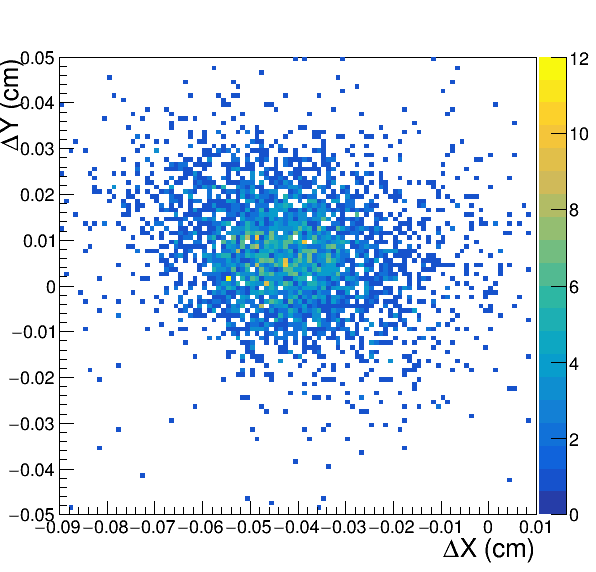
\includegraphics[width=\linewidth]{thesis_figures/alignment/Run_3211_before/square/GEM1.png}

   \caption{GEM1 before alignment}
   \label{fig:GEM1_before}
 \end{subfigure}
 %\hfill
 \begin{subfigure}[r]{.45\textwidth}
   \centering
   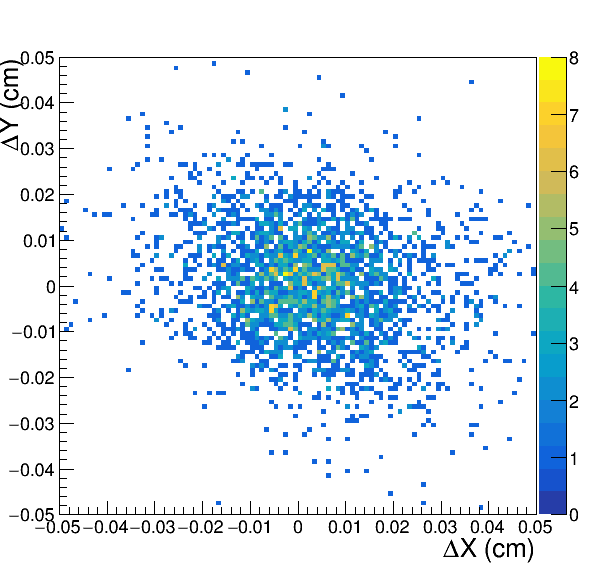
\includegraphics[width=\linewidth]{thesis_figures/alignment/Run_3211_after_millepede/square/GEM1.png}
   \caption{GEM1 after Millepede}
   \label{fig:GEM1_after}
 \end{subfigure}
 \hfill
 \begin{subfigure}[l]{.45\textwidth}
   \centering
   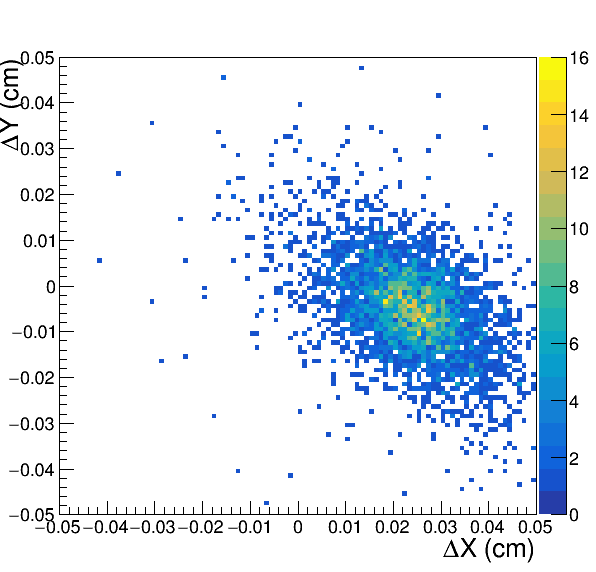
\includegraphics[width=\linewidth]{thesis_figures/alignment/Run_3211_before/square/GEM2.png}
   \caption{GEM2 before alignment}
   \label{fig:GEM2_before}
 \end{subfigure}
 %\hfill
 \begin{subfigure}[r]{.45\textwidth}
   \centering
   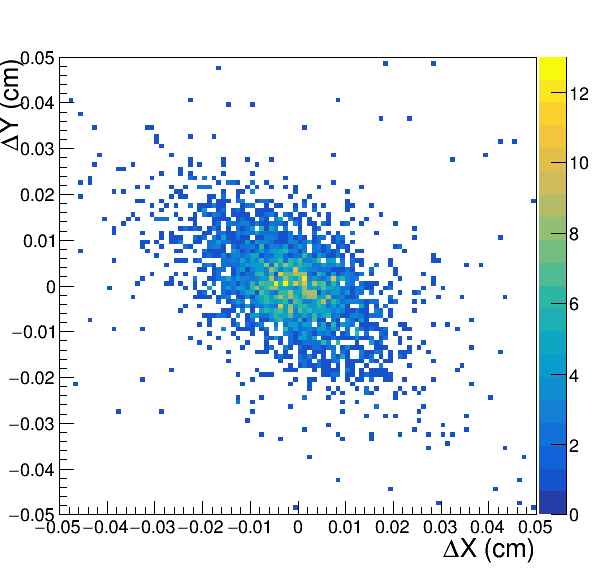
\includegraphics[width=\linewidth]{thesis_figures/alignment/Run_3211_after_millepede/square/GEM2.png}
   \caption{GEM2 after Millepede}
   \label{fig:GEM2_after}
 \end{subfigure}
 \begin{subfigure}[l]{.45\textwidth}
   \centering
   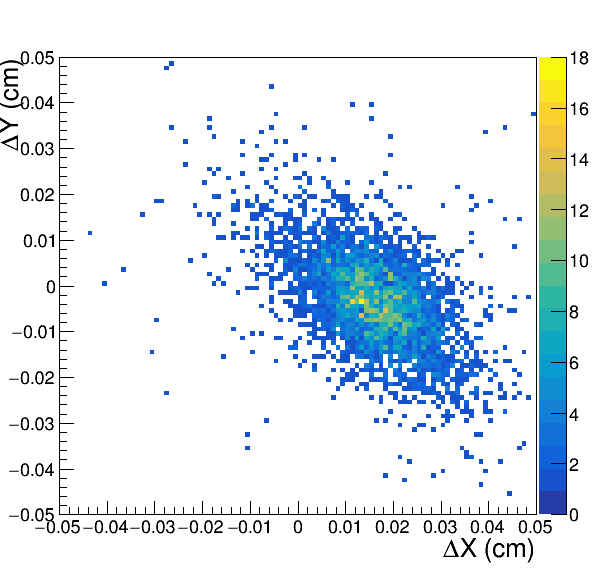
\includegraphics[width=\linewidth]{thesis_figures/alignment/Run_3211_before/square/GEM4.png}

   \caption{GEM4 before alignment}
   \label{fig:GEM4_before}
 \end{subfigure}
 %\hfill
 \begin{subfigure}[r]{.45\textwidth}
   \centering
   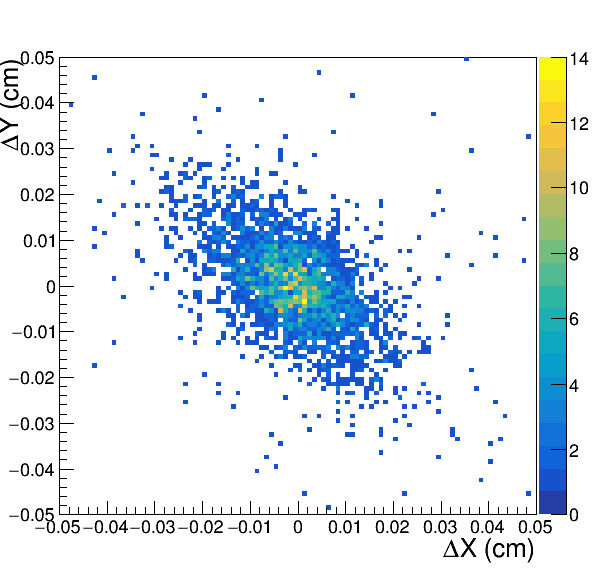
\includegraphics[width=\linewidth]{thesis_figures/alignment/Run_3211_after_millepede/square/GEM4.png}
   \caption{GEM4 after Millepede}
   \label{fig:GEM4_after}
 \end{subfigure}
 \caption{Residual of GEM detectors}
 \label{fig:GEM_residuals}
\end{figure}

%%%%MICROMEGAS start here

\begin{figure}[h!]
\centering
 \begin{subfigure}[l]{.45\textwidth}
   \centering
   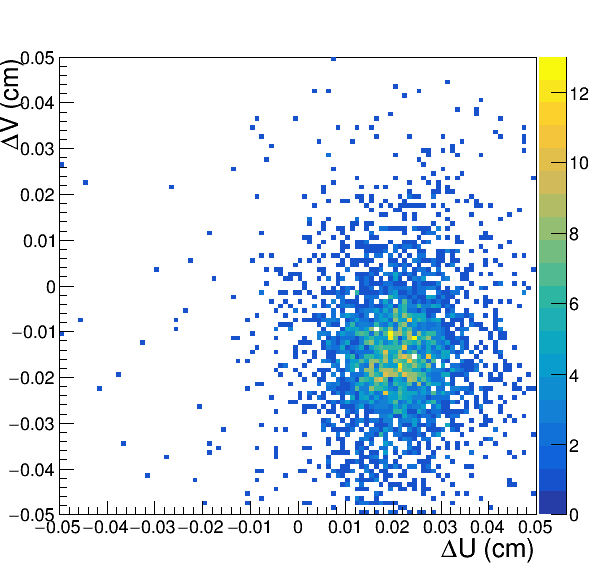
\includegraphics[width=\linewidth]{thesis_figures/alignment/Run_3211_before/square/MX1.png}

   \caption{MM1 before alignment}
   \label{fig:MX1_before}
 \end{subfigure}
 %\hfill
 \begin{subfigure}[r]{.45\textwidth}
   \centering
   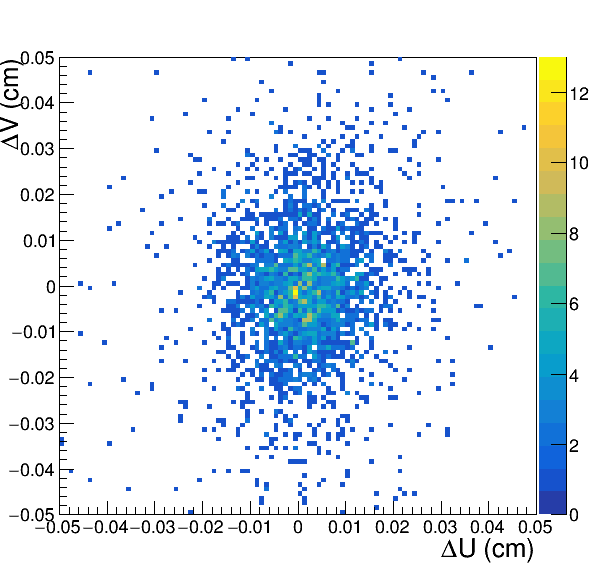
\includegraphics[width=\linewidth]{thesis_figures/alignment/Run_3211_after_millepede/square/MX1.png}
   \caption{MM1 after Millepede}
   \label{fig:MX1_after}
 \end{subfigure}
 \hfill
 \begin{subfigure}[l]{.45\textwidth}
   \centering
   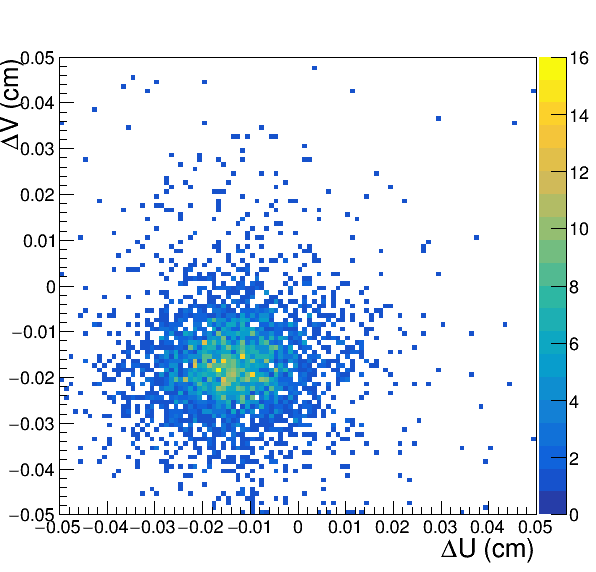
\includegraphics[width=\linewidth]{thesis_figures/alignment/Run_3211_before/square/MX2.png}
   \caption{MM2 before alignment}
   \label{fig:MX2_before}
 \end{subfigure}
 %\hfill
 \begin{subfigure}[r]{.45\textwidth}
   \centering
   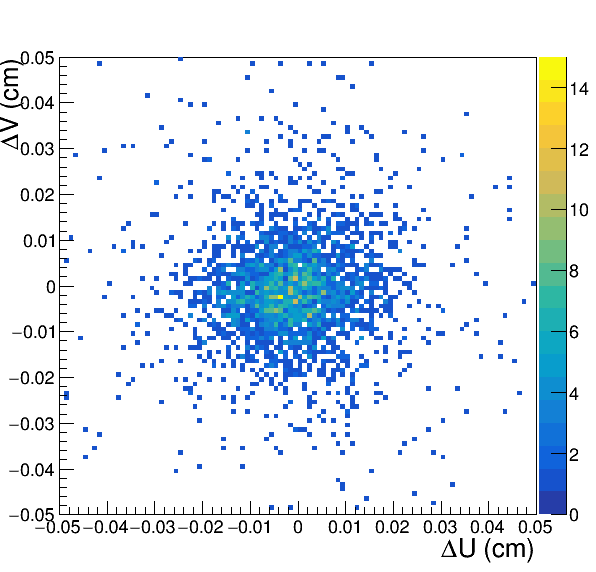
\includegraphics[width=\linewidth]{thesis_figures/alignment/Run_3211_after_millepede/square/MX2.png}
   \caption{MM2 after Millepede}
   \label{fig:MX2_after}
 \end{subfigure}
 \begin{subfigure}[l]{.45\textwidth}
   \centering
   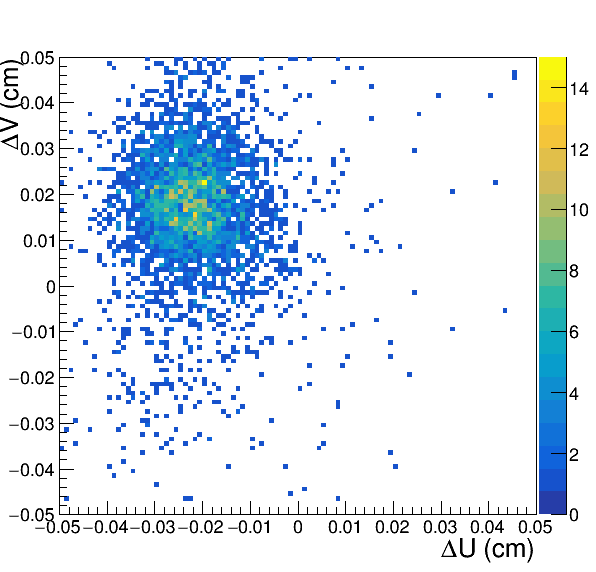
\includegraphics[width=\linewidth]{thesis_figures/alignment/Run_3211_before/square/MX3.png}

   \caption{MM3 before alignment}
   \label{fig:MM3_before}
 \end{subfigure}
 %\hfill
 \begin{subfigure}[r]{.45\textwidth}
   \centering
   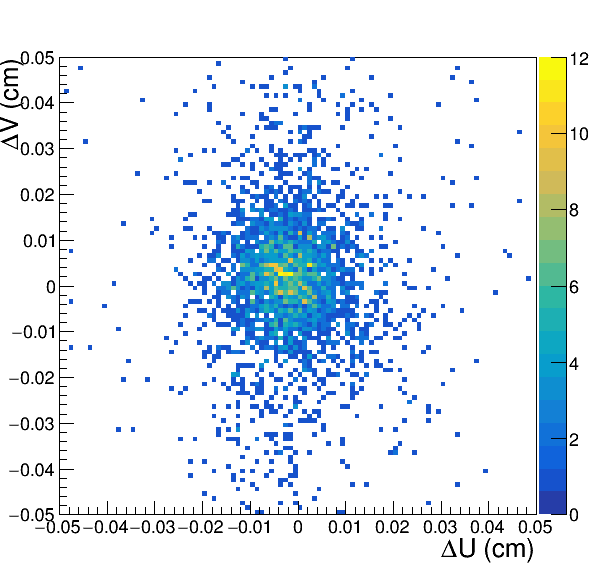
\includegraphics[width=\linewidth]{thesis_figures/alignment/Run_3211_after_millepede/square/MX3.png}
   \caption{MM3 after Millepede}
   \label{fig:MX3_after}
 \end{subfigure}
 \caption{Residual of Micromega detectors}
  \label{fig:MX_residuals_1}
\end{figure}


\begin{figure}[h!]
\centering
 \begin{subfigure}[l]{.45\textwidth}
   \centering
   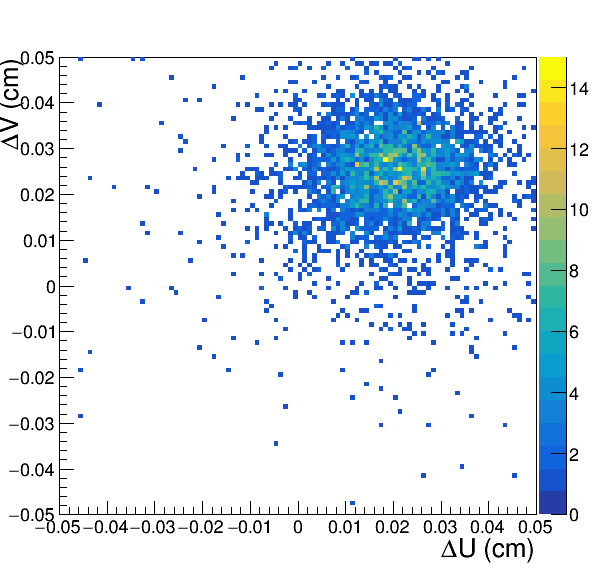
\includegraphics[width=\linewidth]{thesis_figures/alignment/Run_3211_before/square/MX4.png}

   \caption{MM4 before alignment}
   \label{fig:MX4_before}
 \end{subfigure}
 %\hfill
 \begin{subfigure}[r]{.45\textwidth}
   \centering
   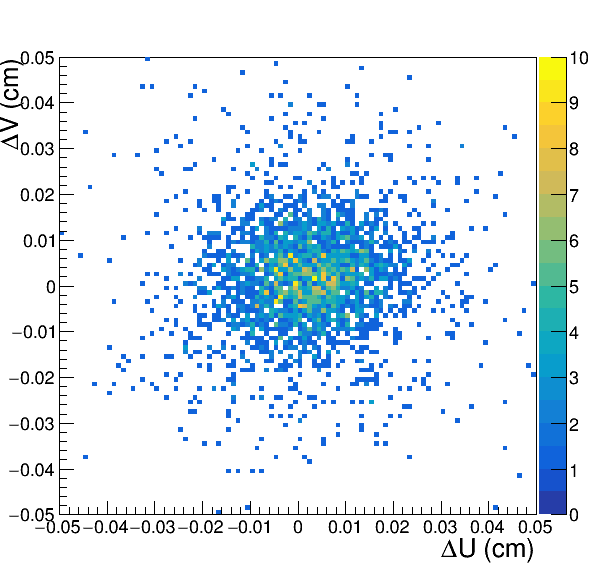
\includegraphics[width=\linewidth]{thesis_figures/alignment/Run_3211_after_millepede/square/MX4.png}
   \caption{MM4 after Millepede}
   \label{fig:MX4_after}
 \end{subfigure}
 \hfill
 \begin{subfigure}[l]{.45\textwidth}
   \centering
   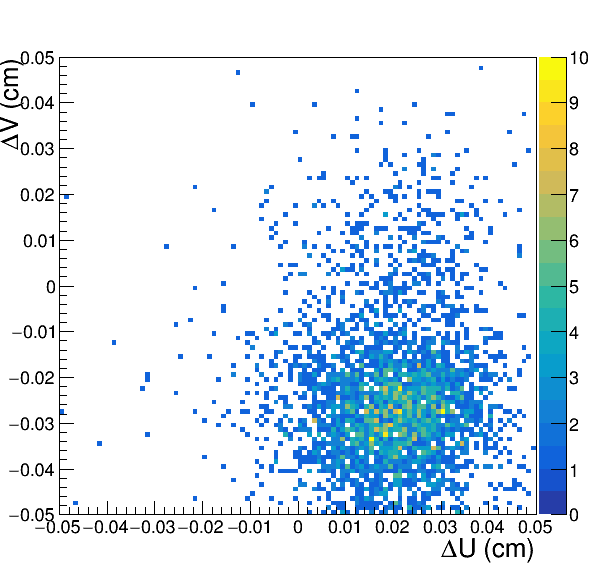
\includegraphics[width=\linewidth]{thesis_figures/alignment/Run_3211_before/square/MX5.png}
   \caption{MM5 before alignment}
   \label{fig:MX5_before}
 \end{subfigure}
 %\hfill
 \begin{subfigure}[r]{.45\textwidth}
   \centering
   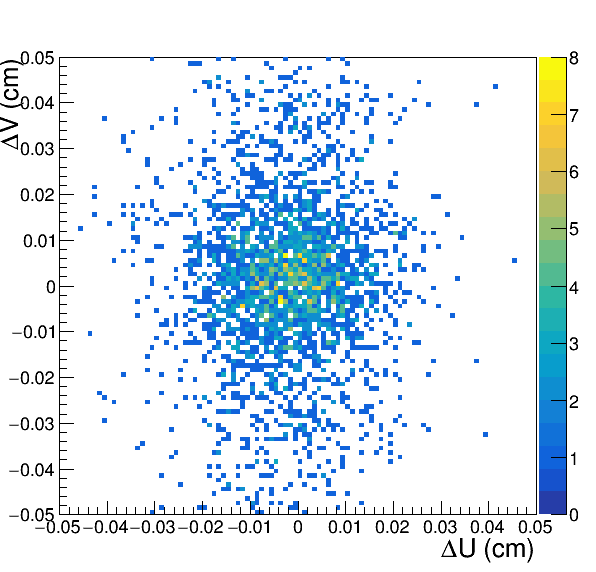
\includegraphics[width=\linewidth]{thesis_figures/alignment/Run_3211_after_millepede/square/MX5.png}
   \caption{MM5 after Millepede}
   \label{fig:MX5_after}
 \end{subfigure}
 \begin{subfigure}[l]{.45\textwidth}
   \centering
   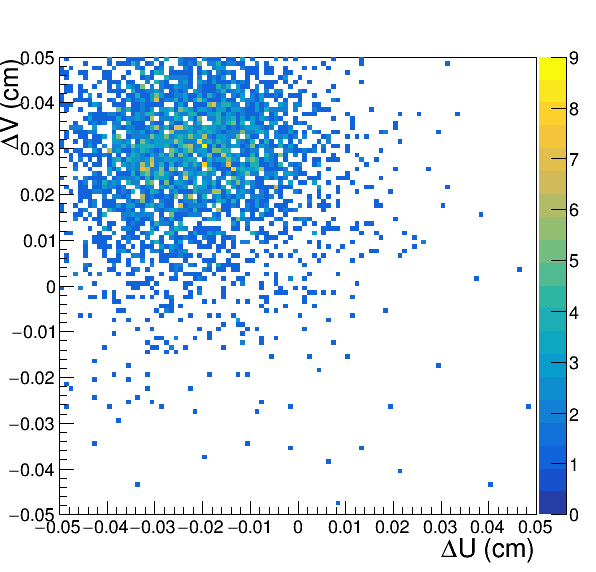
\includegraphics[width=\linewidth]{thesis_figures/alignment/Run_3211_before/square/MX7.png}

   \caption{MM6 before alignment}
   \label{fig:MX6_before}
 \end{subfigure}
 %\hfill
 \begin{subfigure}[r]{.45\textwidth}
   \centering
   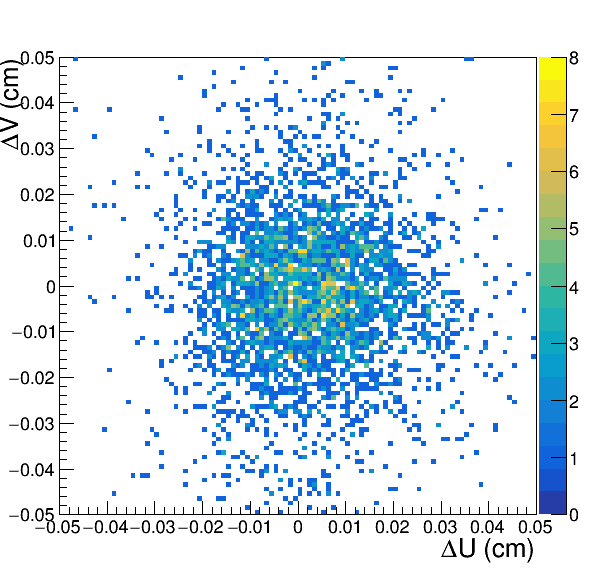
\includegraphics[width=\linewidth]{thesis_figures/alignment/Run_3211_after_millepede/square/MX7.png}
   \caption{MM6 after Millepede}
   \label{fig:MX6_after}
 \end{subfigure}
 \caption{Residual of Micromega detectors}
 \label{fig:MX_residuals_2}
\end{figure}

\begin{figure}[h!]
\centering
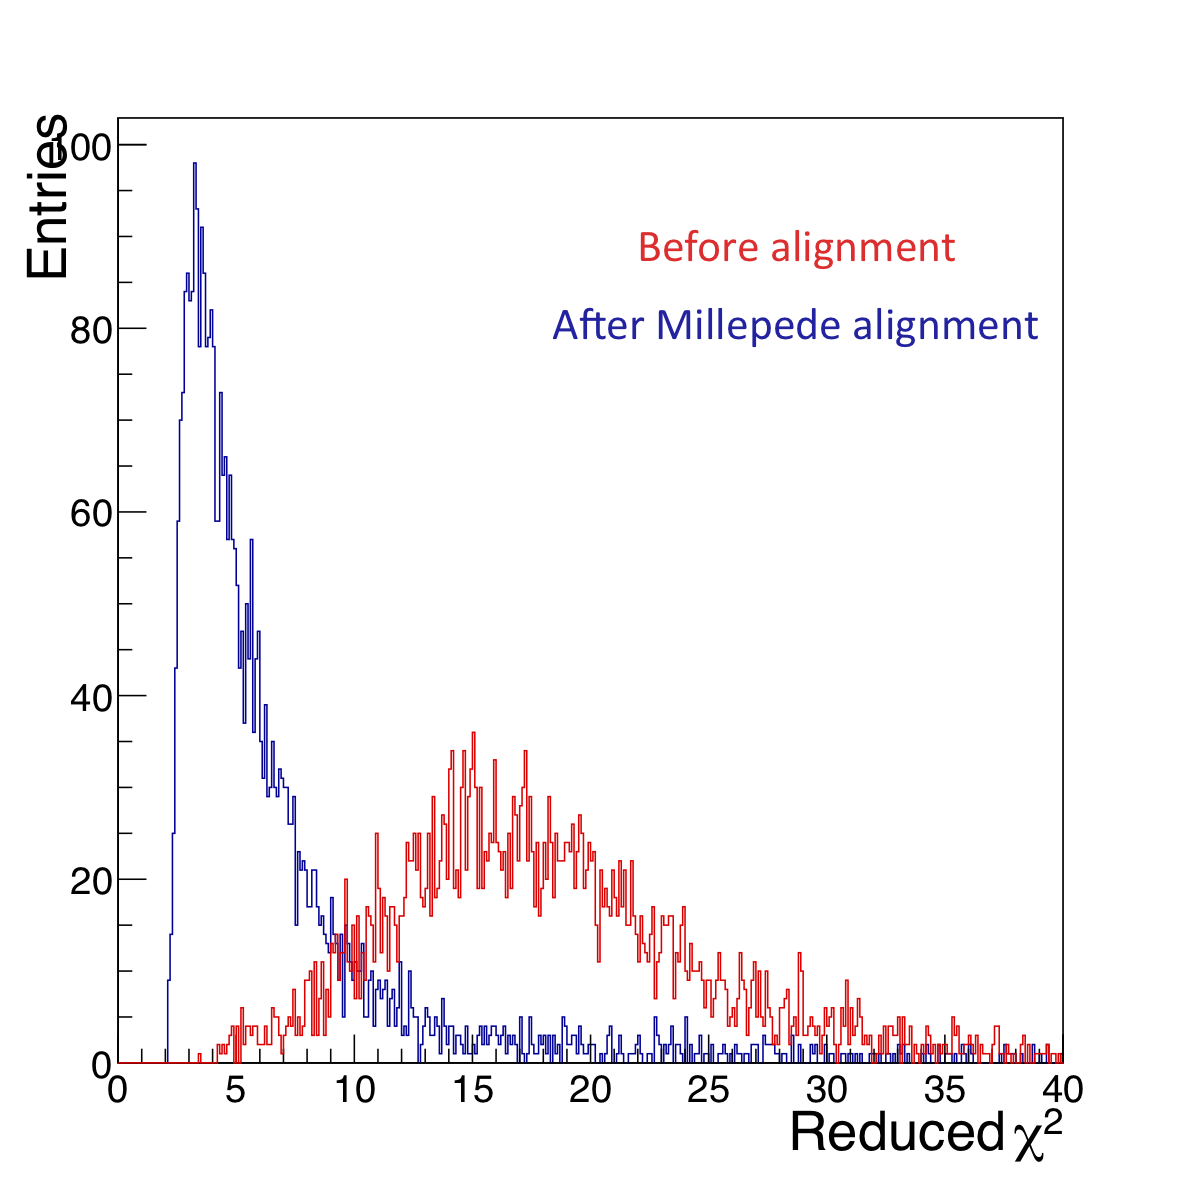
\includegraphics[width=0.6\textwidth]{thesis_figures/alignment/red_chi2_bvs_after_square.png}
\caption{$\chi_{red}^2$ comparison before and after Millepede alignment implementation}
\label{fig:red_chi2_1}
\end{figure}

\begin{figure}[h!]
\centering
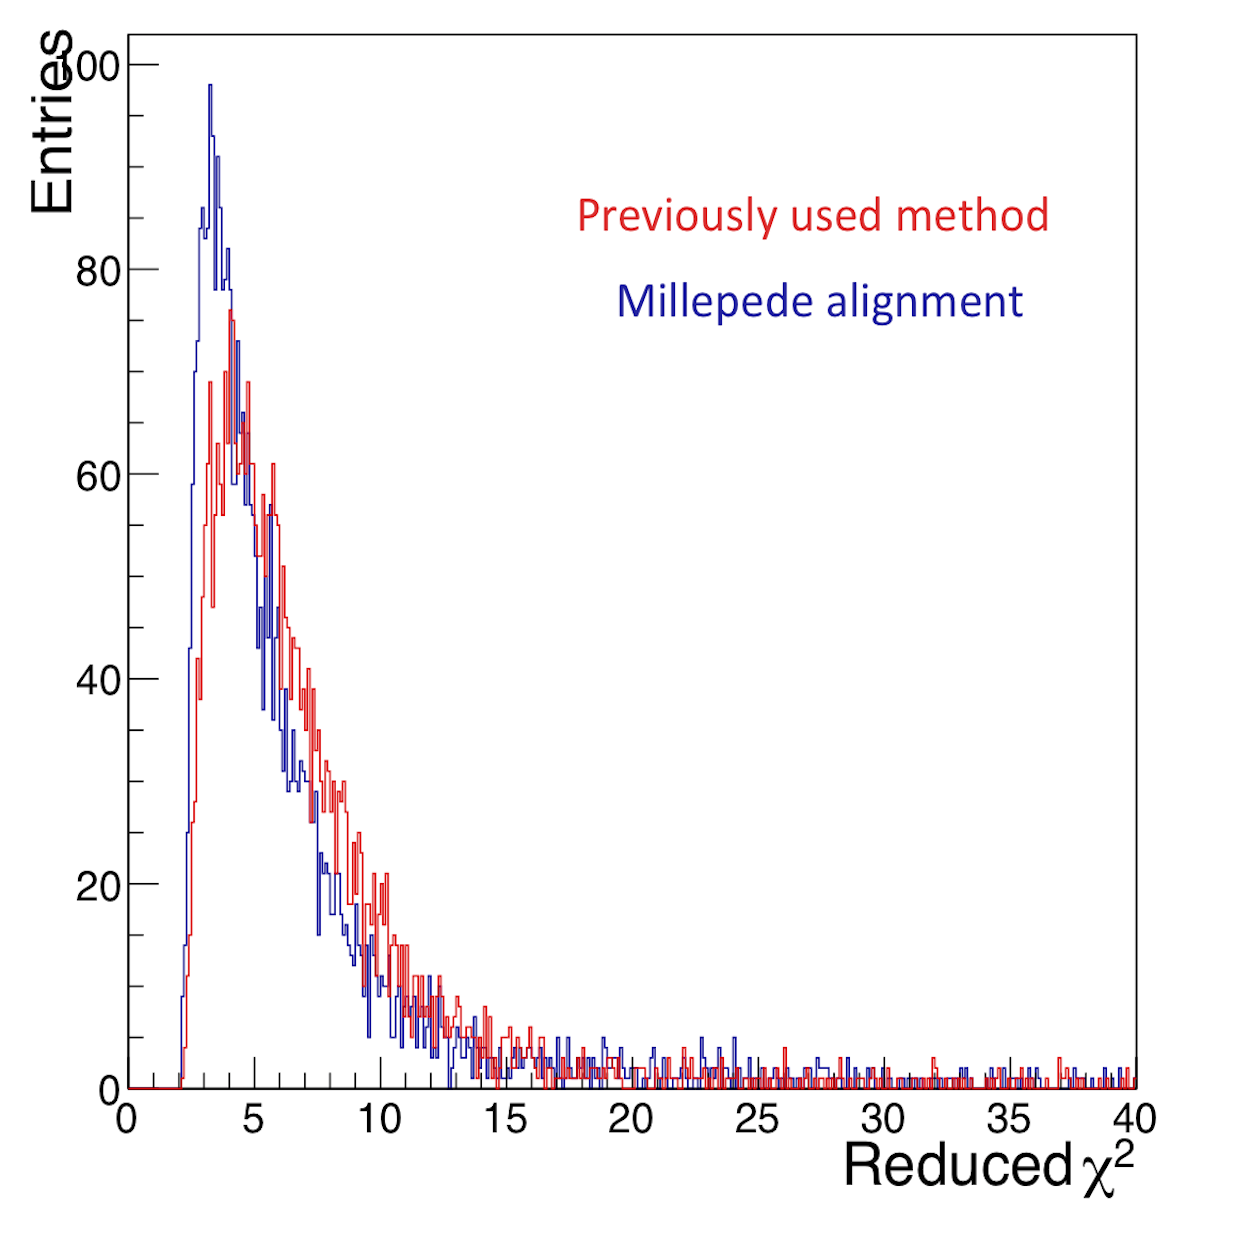
\includegraphics[width=0.6\textwidth]{thesis_figures/alignment/red_chi2_navsm_final.png}
\caption{$\chi_{red}^2$ comparison of previously used method with Millepede alignment implementation}
\label{fig:red_chi2_2}
\end{figure}

%%Micromegas off and not off
\begin{figure}[h!]
\centering
\begin{subfigure}[l]{.45\textwidth}
  \centering
  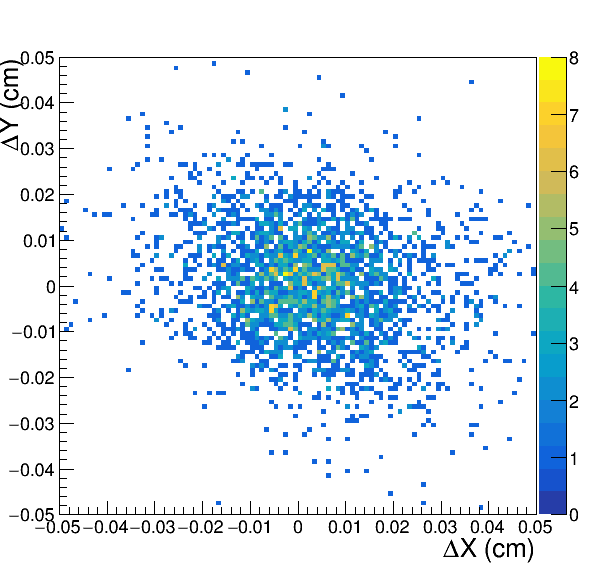
\includegraphics[width=\linewidth]{thesis_figures/alignment/Run_3211_after_millepede/square/GEM1.png}
  \caption{GEM1 after Millepede}
  %\label{fig:GEM1_after}
\end{subfigure}
%\hfill
\begin{subfigure}[r]{.45\textwidth}
  \centering
  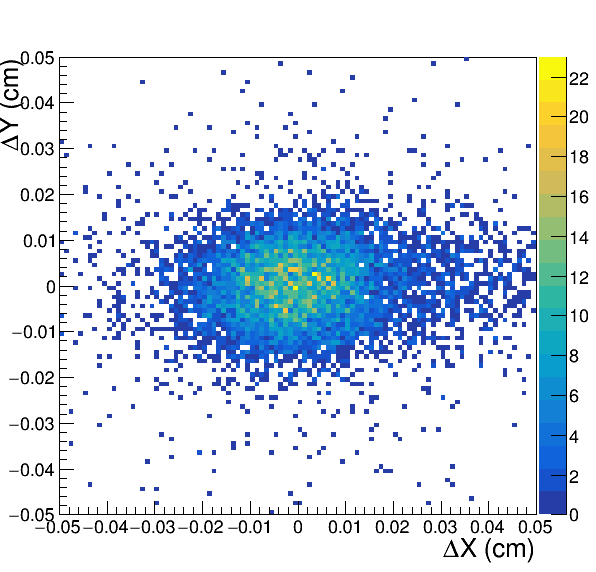
\includegraphics[width=\linewidth]{thesis_figures/alignment/Run_3211_after_millepede/Micromegas_off/GEM1.png}
  \caption{GEM1 after Millepede MM-off}
  \label{fig:GEM1_MXoff}
\end{subfigure}
\hfill
\begin{subfigure}[l]{.45\textwidth}
  \centering
  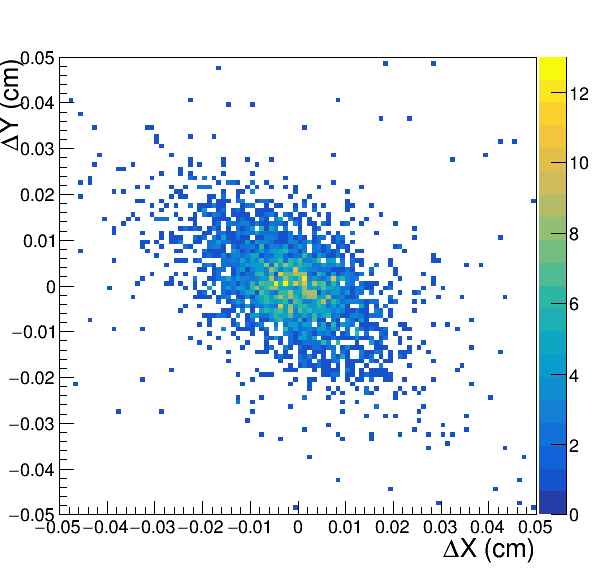
\includegraphics[width=\linewidth]{thesis_figures/alignment/Run_3211_after_millepede/square/GEM2.png}
  \caption{GEM2 after Millepede}
  %\label{fig:GEM2_after}
\end{subfigure}
%\hfill
\begin{subfigure}[r]{.45\textwidth}
  \centering
  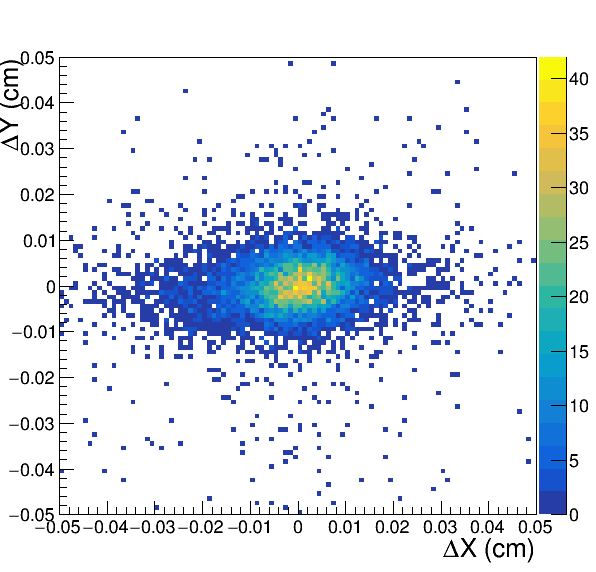
\includegraphics[width=\linewidth]{thesis_figures/alignment/Run_3211_after_millepede/Micromegas_off/GEM2.png}
  \caption{GEM2 after Millepede MM-off}
  \label{fig:GEM2_MXoff}
\end{subfigure}
\begin{subfigure}[l]{.45\textwidth}
  \centering
  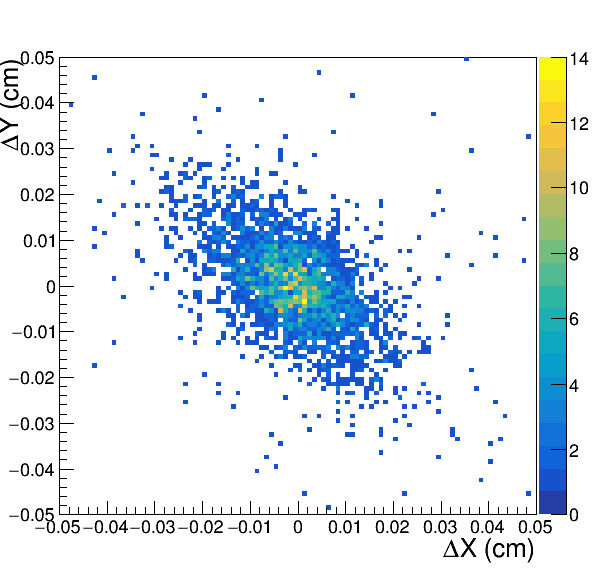
\includegraphics[width=\linewidth]{thesis_figures/alignment/Run_3211_after_millepede/square/GEM4.png}
  \caption{GEM4 after Millepede}
  %\label{fig:GEM4_after}
\end{subfigure}
%\hfill
\begin{subfigure}[r]{.45\textwidth}
  \centering
  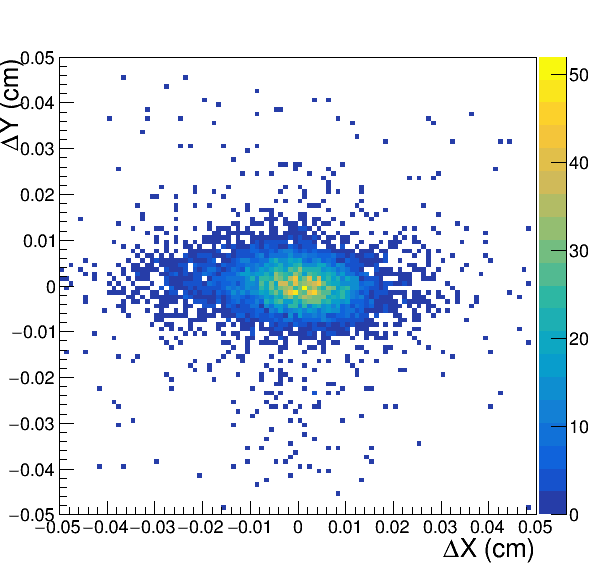
\includegraphics[width=\linewidth]{thesis_figures/alignment/Run_3211_after_millepede/Micromegas_off/GEM4.png}
  \caption{GEM4 after Millepede MM-off}
  \label{fig:GEM4_MXoff}
\end{subfigure}
\caption{Residual of GEM detectors with downstream Micromegas switched off}
\label{fig:MX_off}
\end{figure}
\FloatBarrier

\subsection[Angular Alignment]%
{Angular Alignment} %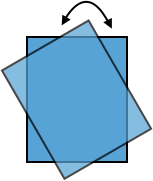
\includegraphics[width=20mm]{thesis_figures/Angular.png}}
Another global parameter that can impact the tracking resolution is the angular displacement. Each plane of the detector has a particular angle with respect to the global reference system. In the case of the GEM detectors used in our setup one plane is at $0^{\circ}$ with respect to the global system and this plane is named the X plane, on the other hand the Y plane, which is the readout plane perpendicular to X is at $90^{\circ}$ w.r.t the global system. This essentially means that the reference system for our GEMs is the same as that of the experiment. In the case of the Micromegas, the internal detector reference system is rotated by $45^{\circ}$ w.r.t the global system. To check whether an angular alignment was needed after the previously performed positional alignment for our setup, the obtained residuals were plotted against the position of hit for each plane of the detector. The results for the GEM detectors are shown in fig.(\ref{fig:res_vs_pos}) while the ones for the Micromegas are given in appendix(\ref{sec:app_1}). It was observed that for most of the detectors the residuals have no dependence on the position except for the case of GEM1, particularly for the X plane. To correct for this dependence an angular alignment was performed.

The angular(T) alignment was performed using the detectors table obtained after six iterations of the positional alignment(U) mentioned before. Initially during the T alignment only the X and Y planes of GEM1 were left free to rotate and all the other detector positions along with their respective angles were fixed. This was done to measure the impact of the alignment for one single detector. GEM1 was chosen since it was seen that the residuals for the X plane of the detector seemed to have a dependence on the position of the hits in the detector. The tracks used for alignment were chosen to have $\chi^2_{red} < 100$ and a $-110 \text{GeV} <\text{p/charge}< -90 \text{GeV}$. The result of the T alignment for GEM1, X plane is shown in fig.(\ref{fig:GEM1_T_align}). As it is seen in the figure the impact of the T alignment is minimal. However, it is important to mention that the result shown here was obtained after three iterations of the Millepede algorithm since the further iterations failed. The failure was during the CORAL part of the procedure which prohibits a change in the angle greater than $5^{\circ}$ for the GEM detectors. In spite of this restriction the three iterations should be more than enough to solve the angular displacement which is not the case. It was also found that the individual X and Y planes of the detector do not stay perpendicular to each other after the T alignment. This is unexpected since even though in CORAL they are treated as separate detectors, in reality the angle between them in the detector reference frame is fixed by construction. The observed angles for the planes were $89.563^{\circ}$ for the Y plane and $-0.324^{\circ}$ for the X plane after alignment i.e there is about a $0.2^{\circ}$ shift in the inherent angle between the two readout planes. This was confirmed to be a possibility which might have arisen during the detector construction particularly the chemical etching process~\cite{SAULI20162} used to construct the readout strips. This might also explain the angular dependence of the residuals observed in GEM1. Fig.(\ref{fig:red_chi2_3}) shows the $\chi^2_{red}$ before and after T alignment. We do see some shift towards a lower value but the overall shape of both the distributions is similar, reiterating the fact that the impact of the angular alignment is minimal for our setup at least in the case where we only align for one detector.

\begin{figure}[h!]
\centering
 \begin{subfigure}[l]{.45\textwidth}
   \centering
   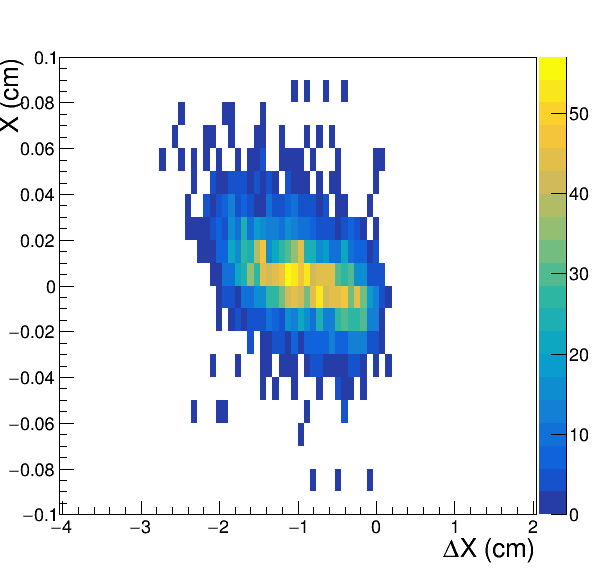
\includegraphics[width=\linewidth]{thesis_figures/alignment/Run_3211_T/G1X_after_millepede_U.png}

   \caption{GEM1 X plane}
   \label{fig:GEM1X_before}
 \end{subfigure}
 %\hfill
 \begin{subfigure}[r]{.45\textwidth}
   \centering
   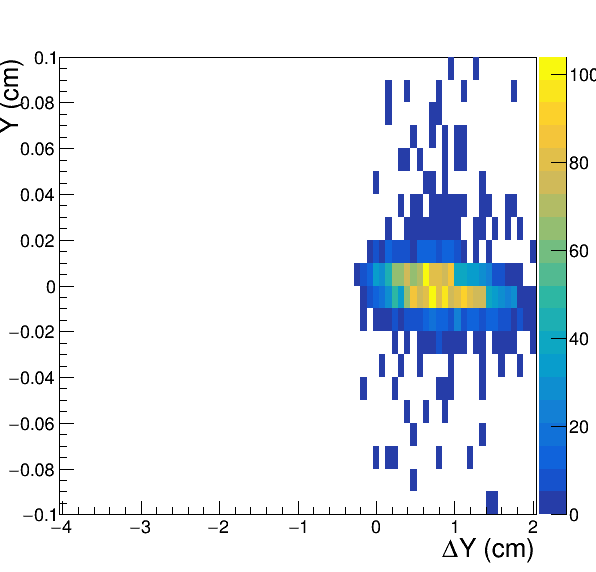
\includegraphics[width=\linewidth]{thesis_figures/alignment/Run_3211_T/G1Y_after_millepede_U.png}
   \caption{GEM1 Y plane}
   \label{fig:GEM1Y_before}
 \end{subfigure}
 \hfill
 \begin{subfigure}[l]{.45\textwidth}
   \centering
   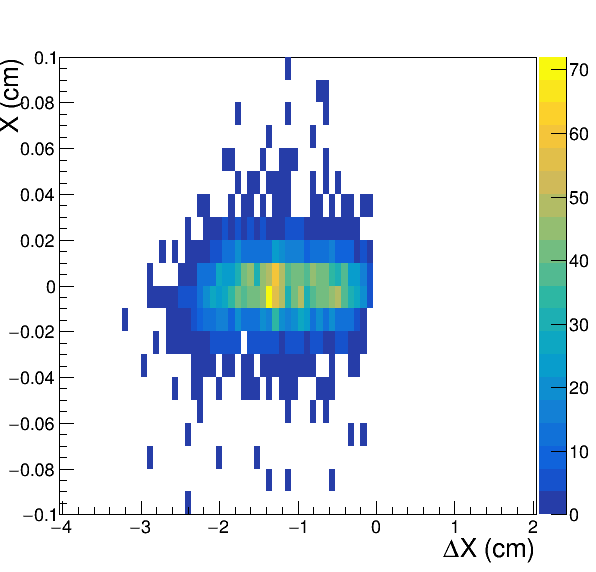
\includegraphics[width=\linewidth]{thesis_figures/alignment/Run_3211_T/G2X_after_millepede_U.png}
   \caption{GEM2 X plane}
   \label{fig:GEM2X_before}
 \end{subfigure}
 %\hfill
 \begin{subfigure}[r]{.45\textwidth}
   \centering
   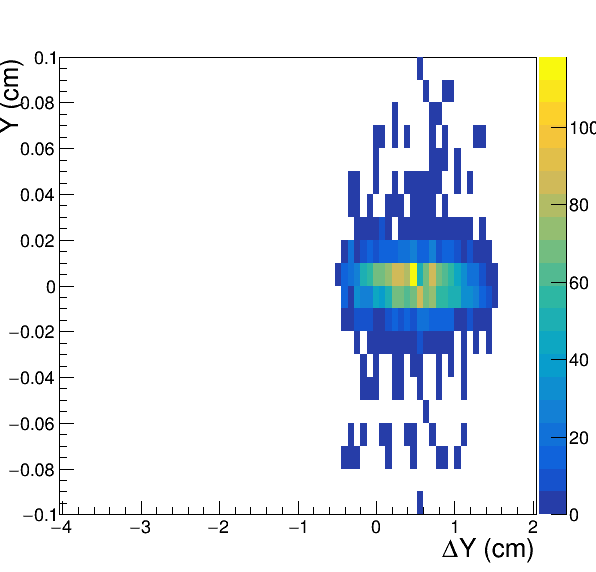
\includegraphics[width=\linewidth]{thesis_figures/alignment/Run_3211_T/G2Y_after_millepede_U.png}
   \caption{GEM2 Y plane}
   \label{fig:GEM2Y_before}
 \end{subfigure}
 \begin{subfigure}[l]{.45\textwidth}
   \centering
   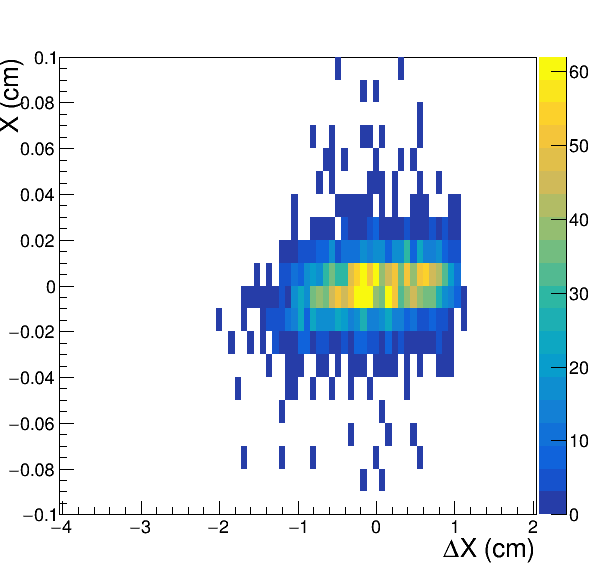
\includegraphics[width=\linewidth]{thesis_figures/alignment/Run_3211_T/G4X_after_millepede_U.png}

   \caption{GEM4 X plane}
   \label{fig:GEM4X_before}
 \end{subfigure}
 %\hfill
 \begin{subfigure}[r]{.45\textwidth}
   \centering
   \includegraphics[width=\linewidth]{thesis_figures/alignment/Run_3211_T/G4Y_after_millepede_U.png}
   \caption{GEM4 Y plane}
   \label{fig:GEM4Y_before}
 \end{subfigure}
 \caption{Residual vs position for GEM detectors}
 \label{fig:res_vs_pos}
\end{figure}

%GEM1X plane alignment

\begin{figure}[h!]
\centering
 \begin{subfigure}[l]{.45\textwidth}
   \centering
   \includegraphics[width=\linewidth]{thesis_figures/alignment/Run_3211_T/G1X_after_millepede_U.png}

   \caption{GEM1 X plane before angular alignment}
   %\label{fig:GEM1X_before}
 \end{subfigure}
 %\hfill
 \begin{subfigure}[r]{.45\textwidth}
   \centering
   \includegraphics[width=\linewidth]{thesis_figures/alignment/Run_3211_T/G1X_after_millepede_T.png}
   \caption{GEM1 X plane after angular alignment}
   \label{fig:GEM1X_after_T}
 \end{subfigure}
 \caption{Angular alignment}
 \label{fig:GEM1_T_align}
 \end{figure}

 \begin{figure}[h!]
 \centering
 \includegraphics[width=0.8\textwidth]{thesis_figures/alignment/red_chi2_T.png}
 \caption{$\chi_{red}^2$ comparison before and after Millepede T alignment implementation}
 \label{fig:red_chi2_3}
 \end{figure}
\FloatBarrier

\subsection{Positional+Angular Alignment}
The end goal with the whole alignment procedure is to obtain the best possible alignment for each detector. Hence, the procedure was studied with both U and T alignment turned on.
Since the slight shift in the angle which was observed during U alignment was only present in a small number of detectors and is more prominent in GEM1 the impact of a U+T alignment was similar to that of U alignment. This alignment was performed just to check whether the alignment algorithm works if multiple global parameters are minimized in unison. The alignment was observed to be operational and the $\chi^2_{red}$ obtained was similar to that shown in fig.(\ref{fig:red_chi2_1}). The impact of the T alignment might not be visible for the particular run that was analyzed since the angular displacement for the detectors was minimal. However, for a future run by run alignment a full U+T alignment should be performed to correct for any possible angular displacement since for NA64 the experimental setup is constantly changing.

%%% Local Variables:
%%% mode: latex
%%% TeX-master: "mythesis"
%%% End:

% !TEX root = mythesis.tex

%==============================================================================
\chapter{Monte Carlo simulation}
\label{sec:MC}
%==============================================================================
The MC simulation for NA64 visible mode for the 2018 setup has been implemented by the collaboration in GEANT4. The information from the MC simulation is currently reconstructed in a standalone reconstruction program similar to how it is done for real data. This chapter tries to document how the simulation is implemented. This is an important facet since the type of process we are trying to study is not part of the SM and is required to be implemented as an extra step to a standard GEANT4 simulation. Though these processes were added in the physics code~\cite{Gninenko:2017yus,PhysRevD.97.072002} it is still important to document how they are included in a simulation.

Since one of the main goals is to implement the data analysis chain in CORAL, reconstructing the MC simulation output (MCTruth) in CORAL is a part of this goal. Thus, the chapter also details the changes made to the MCTruth to make it compatible with CORAL along with the results of the said reconstruction.

\section{$A'$ Production}
$A'$ production in the NA64 simulation has been described in~\cite{Gninenko:2017yus}. A short summary for the procedure is as follows:
\begin{description}
  \item $-$ The emission probability for $A'$ production for an active target which in our case is fixed to be Pb is given as $P_{emission} = \rho N_A \sigma_{tot}^{A'} \Delta L_i / A $ where $\rho$ is the density of the target, $N_A$ is the Avogadro's number, $\sigma_{tot}^{A'}$ is the total cross-section for the $A'$ production in a bremsstrahlung like reaction as mentioned before, $\Delta L_i$ is the step length of the electron path in the target and $A$ is the atomic weight.

  The total cross-section is approximated by using IWW approximation however as it is seen in the fig.(\ref{fig:ETLvsIWW}), ETL calculation is more accurate and complete. The error in the cross-section calculation is fixed by introducing a K-factor defined as $K = \sigma_{IWW}^{A'} / \sigma_{ETL}^{A'}$.

  \item $-$ A sample variable $u_1$ is randomly sampled from a uniform distribution over the unit interval [0,1]. If $u_1$ is found to be smaller than the emission probability $P_{emission}$ the the simulation for $A'$ proceeds further.

  \item $-$ For an $A'$ emission a random picking for the relevant kinetic parameters $x$, $cos\theta$ and the azimuthal angle $\phi$ is done. The simulation for $A'$ emission and decay continues if the parameters are accepted after rejection sampling.

  \item $-$ Next the kinetic energy for the emitted $A'$ is set. Based on this value it is checked whether at the simulated $A'$ mass the dark photon can escape the subsequent WCAL catcher which is directly after the active target for the visible mode. If this is true then the $A'$ is simulated to decay into $e^+e^-$ and the relevant information about $A'$ and the decay particles which include mass, decay position and momentum is recorded.
\end{description}

\begin{figure}[t!]
\centering
\includegraphics[width=12cm]{thesis_figures/IWWvsETL.png}
\caption{Number of simulated signal events at two $A'$ masses as a function of Dark Photon energy~\cite{Gninenko:2017yus}}
\label{fig:ETLvsIWW}
\end{figure}

\section{Tracking Detectors}
NA64 consists of two sets of tracking detectors namely Micromegas and GEMs. In the visible mode simulation two Micromegas named MM1 and MM2 are placed upstream of the two magnets and two more named MM3 and MM4 are placed right after the vacuum tube and before the WCAL. Four additional GEM detectors are placed right after the downstream WCAL. Both GEMs and Micromegas have the same implemented internal structure in the simulation. The structure consists of an Argon gasbox surrounded by two Mylar layers on either side. An additional layer of Copper and PCB is added after the second Mylar layer. The gas volume is set as sensitive for both Micromegas and GEMs.

While processing the output of the simulation for the tracking detectors the following information about each particle traversing the detector is recorded- x,y and z hit positions, energy deposited, trackID of the particle, the PDG~\cite{pdg2010} encoding of the particle and the kinetic energy. The trackID is a unique ID which GEANT4 gives to each particle simulated and tracked during the simulation. The trajectories and the origin of \emph{all} the simulated and tracked particles are not saved in the current format. Some trajectories such as those of the beam particle and the simulated $A'$ along with its decay products is available. Saving all trajectories should be considered in the future since the information is useful for reconstruction.

To reconstruct the simulation output it was modified to a format that can be read in CORAL described more in appendix(\ref{sec:app_2}). This comprised of including information such as a unique identifier for each tracking detector (Detector name + DetectorID), particle trajectories for relevant simulated particles and splitting the information to individual detector planes for implementation in CORAL. Additional options were provided in the track fitting option files to activate MC decoding. The reconstruction in GEMs proceeds in the following way:
\begin{enumerate}
  \item For an event CORAL reads in the hit positions for the individual detectors and checks the validity of the TrackIDs against provided trajectories.
  \item Next it moves on to the detector response simulation where it uses the hit data along with extra simulation parameters to simulate three amplitudes for each detector. The simulation parameters include space resolution of the detector (mm), effective gain of the detector along with the standard deviation, signal width (mm) and time resolution (ns) if the timing information is available. The simulation parameters are fed through the track option file.
  \item The simulated amplitude is calculated as follows, $ amp = \frac{1}{\sqrt{2\pi}}\frac{(\text{Energy~deposited} \times (\text{Effective gain} + \sigma_{\text{Gain}}))^2}{\text{signal width}} $ with inbuilt cuts to remove meaningless hits.
  \item The simulated amplitude for the hit is then assigned to the nearest readout strips it might corroborate to.
  \item The amplitudes for each strip are then passed to clusterization and tracking.
\end{enumerate}
The reconstruction for the tracking detectors is evaluated by looking at the reconstructed momentum.

\section{Calorimeters}
 As mentioned before, NA64 consists of three types of calorimeters namely WCAL, ECAL and HCAL in the visible mode setup. The WCAL is simulated to consist of three layers similar to the real setup. These are the pre-shower, main and the catcher. After the simulation the total energy deposited in each layer is calculated for each simulated event. The ECAL also has the same structure in GEANT4 simulation as that of the experiment. It is separated into two layers of 6x6 cells each. Lastly, the HCAL consists of 4 modules with 3x3 cells each. These modules are shifted incrementally in the x position to cover the angle acquired by the beam after it passes through the magnets. Unlike the real setup the last module is not placed in the line of sight of the incoming beam before the magnets. Especially for ECAL and HCAL only the total energy deposited in each cell for each simulated event is processed. No other information regarding the hit positions of the particles that go through the calorimeters is collected.

 The required format for calorimeters so that they can be read and reconstructed in CORAL is the same as the tracking detectors. An example of the formatted simulation output which was fed to CORAL along with its description is given in the appendix(\ref{sec:app_2}). During the reconstruction, the simulated data is just pushed through without any changes for all the calorimeters. Clusterization and track matching is not done since the opening angle of the $e^+e^-$ pair produced due to the decay of $A'$ is expected to be very small such that the currently used dimensions of the individual cells in the ECAL cannot separate the individual particle showers. This leads to the shower being contained within a minimum of one and maximum of two cells if the particle hits the boundary. Hence clusterization makes no sense. This fact is reiterated by the reconstruction results. In addition, since we have no information regarding the individual hit positions track matching cannot be performed in the current reconstruction. However, to study rare SM events such as dimuon production a clusterization in the HCAL to detect individual muon showers may be required.

 % The signature for a dark photon production and decay in the visible mode if we just use the information available from the calorimeters is: "Energy deposited WCAL + Energy deposited ECAL = Beam energy". Additionally, no energy should have been deposited in the HCAL i.e the total shower of the decay products is contained in the ECAL.


 \section{Trigger Detectors}
 This category includes detectors like the SRD, Vetos, Scintillators and Counters. In the 2018 simulation the SRD, VETO in front of the HCAL along with Wcounters(W0-2) were replicated. The SRD is split into SRD counters in the transverse direction similar to the one in the real setup (fig.(\ref{fig:Visible_mode_setup_side})). The MC simulation consists of two counters instead of the three present in the real setup.

 For this class of detectors only the information regarding the total energy deposited in the detector is important. Hence, during the reconstruction similar to the calorimeters, this information is pushed through for each detector. The reconstructed data for the triggers and the SRD can then be used in the further analysis by applying similar cuts on the energy deposited as that of the real data.
\newpage
\section{Reconstruction Results}
All of the studies mentioned below offer a proof of principle that the MC reconstruction in CORAL is operational and can be used in a more detailed analysis if required.

Fig.(\ref{fig:CORAL_display}) shows the track reconstruction display output from CORAL along with a few modifications to depict the simulated detectors. The blue lines in the figure represent the measured magnetic field maps of the two magnets, the blue loops depict the change in magnetic field and the uncolored region signifies a uniform field in that area. The pink track on the left is the trajectory of the beam particle which hits the upstream Micromegas (MM1-MM2). The first orange track which ends at the downstream Micromegas (MM3-MM4) is used to extract the momentum of the incoming beam. These are studied in more detail in section(\ref{subsec:mom_reco}). Further the energy deposited in the WCAL and the Wcounters (W0-2) is recorded. The event which is being shown here is one where a Dark Photon was produced. This was checked by looking at the sum of energy deposited in the calorimeters and the two tracks reconstructed in the four GEM detectors located after the WCAL. The two tracks are of the corresponding decay products of the $A'$ which are the $e^+ e^-$. These events are described more in section(\ref{subsec:a'_reco}).
 \begin{figure}[t!]
 \centering
 \includegraphics[width=\textwidth]{thesis_figures/MC_reco/CORAL_display_2.png}
 \caption{Track reconstruction display from CORAL.}
 \label{fig:CORAL_display}
 \end{figure}

\subsection{Momentum Reconstruction}
\label{subsec:mom_reco}
The momentum reconstruction in CORAL was checked by selecting the reconstructed tracks which were bridged through the magnets successfully. It was made sure that all tracking detectors upstream and downstream that are involved in momentum reconstruction had a contribution to the track i.e each detector had a hit which was used to reconstruct the final fitted track. In our case this meant the four Micromega detectors.
 \begin{figure}[h!]
 \centering
 \includegraphics[width=0.9\textwidth]{thesis_figures/MC_reco/beam_mom_bigger_axis.pdf}
 \caption{Reconstructed beam momentum in CORAL along with fit parameters.}
 \label{fig:reco_beam_mom}
 \end{figure}

Fig.(\ref{fig:reco_beam_mom}) shows the reconstructed beam momentum. The momentum was fitted with a standard Gaussian function. The extracted momentum after reconstruction has a value of $146.4 ~\text{GeV}$ with an error of $2.58 ~\text{GeV}$. Even though we have a beam which has a momentum of $150 ~\text{GeV}$ after simulation, we observe that the reconstructed beam momentum is much lower. Since the detectors in the reconstruction were placed at the exact position as that of the simulation, the reason for the observed beam momentum distribution can be either attributed to the difference in the integrated magnetic field between the simulation and the reconstruction or it can also be due to some systematic error of the track reconstruction and momentum determination algorithm. The Gaussian spread in the reconstructed momentum should be due to the resolution of the detectors mimicked in the reconstruction.

The magnetic field in the simulation is implemented as a box field with an integrated field strength of $7.85~\text{Tm}$ while in the reconstruction the measured field maps of the magnets made for the physics runs are used. Even though the integrated magnetic fields for both the implementations are almost the same the bending effect which might be present due to the fringe fields is only simulated during the reconstruction. This might be the reasons for the the underestimation of the calculated beam momentum compared to the one simulated.

To check the performance of the tracking algorithm for momentum reconstruction the angles of the incoming track were compared to the fitted momentum after track fitting. Figures (\ref{fig:reco_mom_dip}) and (\ref{fig:reco_mom_azi}) show the obtained result. Both of the angles are chosen from the fitted track piece which is upstream of the magnet. The dip angle is defined as the angle of the track which moves it in a plane parallel to the magnetic field lines hence during the bending process this angle is not affected and does not contribute to the momentum reconstruction. As seen in the fig.(\ref{fig:reco_mom_dip}) the fitted momentum over the distribution of the dip angle is uniform which is as expected.

The azimuthal angle is the angle of the track piece which moves it in a direction perpendicular to that of the magnetic field. This is the angle affected by the bending field of the magnet and is critical for momentum reconstruction. As we see in fig.(\ref{fig:reco_mom_azi}) there is a correlation between the fitted momentum and the incoming track's azimuthal angle. This shows that during the reconstruction, tracks with varying azimuthal angles were reconstructed which led to a spread in the reconstructed beam momentum. This might add some systematic uncertainties to the beam momentum observed and should be investigated further examining the reconstruction algorithm in CORAL in future studies.

 \begin{figure}[t!]
 \centering
 \includegraphics[width=\textwidth]{thesis_figures/MC_reco/mom_vs_dip.pdf}
 \caption{Fitted beam momentum vs dip angle of incoming track. }
 \label{fig:reco_mom_dip}
 \end{figure}

 \begin{figure}[h!]
 \centering
 \includegraphics[width=\textwidth]{thesis_figures/MC_reco/mom_vs_azi.pdf}
 \caption{Fitted beam momentum vs azimuthal angle of incoming track.}
 \label{fig:reco_mom_azi}
 \end{figure}
\newpage

 \subsection{A' Reconstruction}
 \label{subsec:a'_reco}
The $A'$ reconstruction in CORAL was looked at in two stages. The first included identifying the $A'$ events in the reconstructed sample and the second included studying the decay products of the $A'$ which are the $e^+ e^-$.

The $A'$ events were selected by applying the following cuts:
\begin{enumerate}
  \item $142~\text{GeV} < E_{WCAL} < 150~\text{GeV} $.
  \item $E_{W_{0-2}}, E_{ECAL} > 0~\text{GeV}$.
  \item Two tracks in downstream GEM detectors.
  \item $E_{VETO} = E_{HCAL} = 0~\text{GeV} $.
\end{enumerate}

These cuts helped separate the $A'$ events from the rare dimuon events mentioned before. The angular distribution of the two track events were analyzed and is shown in fig.(\ref{fig:reco_angle}). The figure shows that most of the $e^+ e^-$ pairs produced from the decay of $A'$ have a small outgoing angle. This is as expected since we assume that the $A'$ which might be produced in a real physics event might be highly boosted in the forward direction which will result in a smaller opening angle for the decay products. The current expected limit for this opening angle for $1 \lesssim m_{A'}\lesssim 25 \text{MeV}$ at $E_{A'}=$20~GeV is $\theta \ll 2\text{mrad}$ as mentioned in~\cite{Banerjee_2018}. This also validates our reasoning to not implement shower clusterization in the downstream calorimeters since at such small angles, with the current size of our individual calorimeter cell, the shower will not achieve the necessary separation required for identifying individual particles.
\FloatBarrier
%\clearpage
 \begin{figure}[t!]
 \centering
 \includegraphics[width=\textwidth]{thesis_figures/MC_reco/ang_dist_final.pdf}
 \caption{Angle between the outgoing $e^+e^-$ tracks}
 \label{fig:reco_angle}
 \end{figure}


%%% Local Variables:
%%% mode: latex
%%% TeX-master: "mythesis"
%%% End:

% !TEX root = mythesis.tex

%==============================================================================
\chapter{Conclusion and Outlook}
\label{chap:conc}
%==============================================================================
% \begin{figure}[h!]
% \centering
% \includegraphics[width=0.85\textwidth]{thesis_figures/chi2_comp_conclusion_2.png}
% \caption{$\chi^2_{red}$ distribution for selected tracks showing the impact of Millepede alignment.}
% \label{fig:red_chi2_4}
% \end{figure}

Besides detecting ultra-high-energy (UHE) cosmic rays, the Pierre Auger Observatory with its large Surface Detector (SD) array offers a remarkable exposure to neutrinos above $10^{17}$eV. Any potential observation of such UHE$\nu_s$ will further our knowledge about the known universe. Since neutrinos are not deflected as they travel towards us at Earth, they offer a direct line of sight to the sources where they were produced. They are also some of the earliest particles produced in a transient source which makes their detection an important beacon for other astronomical instruments to perform a multi-messenger observation. The Pierre Auger Observatory is constantly monitoring the sky for the presence of such UHE$\nu_s$. The idea behind the detection remains the same as previous analysis at Auger where the neutrinos are assumed to induce Extensive Air Showers (EASs) close to the ground with a large electro-magnetic component at ground ("young" showers). This strategy is only employed for horizontal showers ($\theta > 60^{\circ}$). Two new SD triggers, time-over-threshold-deconvolved (ToTd) and multiplicity of positive steps (MoPS) were installed in 2014 to further increase the detection efficiency for low energy neutrino induced EASs. This thesis presents the first analysis of this improved efficiency for low energy neutrino showers in the zenith range $\theta \in [60^{\circ},75^\circ]$ also known as Down-going low or DG$_{Low}$ range. In this thesis the effect of the new triggers was evaluated for two types of searches, the searches for the diffused flux of UHE$\nu_s$ and search for point-like sources of UHE$\nu_s$. For both searches an overall improvement of efficiency is observed when information from the new triggers is incorporated in the analysis. A short summary of the three main contributions of this thesis along with an outlook detailing potential improvements are detailed in the next sections. 
\section*{Incorporating new triggers in the DG$\mathrm{_{low}}$ UHE$\nu_s$ searches}
During this thesis each facet of the DG$_{low}$ analysis was analysed. An effort was made to maximize the potential of the analysis. A blind search strategy similar to~\cite{gap_note_2013,Aab_2019_diffuse} was followed to avoid any bias in the analysis. The first step in this process was to include the information from the new triggers in the neutrino searches. About $\sim$7 years of recorded data was available for this task. The effect of the new triggers was first evaluated on neutrino simulations by including them in the analysis chain as described in section~\ref{subsubsec:nu_sel_fisher_training}. By the inclusion of new triggers an overall increase in reconstructed events was observed as shown in fig~\ref{fig:Events_vs_angle_summary}. This increase was most significant for lower energy neutrinos and decreased with increase in primary energy. This was an expected consequence due to the design of the new triggers. The overall increase also allowed for further modifications to the analysis which included lowering some stringent cuts as described in section~\ref{subsec:nu_sel_nudeteff}. For the final step of the analysis a Fisher discriminate polynomial was built and trained using the simulations (signal training sample) and a small fraction of recorded data, $\sim$20\% from the Observatory (background training sample). The polynomial is built with Area over Peaks (AoPs) of the stations and a differentiation between the background and signal is performed based on a cut on the Fisher value as given in eq.~\ref{eq:fisher_poly_cut}.
After the fixing the selection, a test sample was unblinded to catch any remaining flaws in the analysis. This proved worthwhile as a small error in the reconstruction was discovered during this process. The error was promptly corrected, and the whole selection procedure was re-evaluated, and the Fisher was retrained. Since the correction involved a change to the reconstruction procedure the blind search was redone from the start. After this correction the unblinding was again performed in two stages. The new test sample and the full blinded sample, 20\% + 60\% of recorded data between the period of 1 Jan 2014 to 31 December 2012 was analysed to search for neutrinos. \textbf{No neutrino candidates} were found in the search performed using the analysis described in this thesis. 

\subsection*{Outlook}
Even though a concerted effort was made to maximize the potential of the analysis presented in this thesis certain improvements could not be implemented and are thus summarized here for future studies. The segmentation algorithm used for reconstruction of events for neutrino searches was found to be not properly tuned for the new triggers, ToTd and MoPS. Thus, for this analysis the new triggers were completely removed from the segmentation algorithm. The primary purpose of the segmentation algorithm is to evaluate the correct start times for the WCD signals to decrease the effect of accidental muons which in turn affects the zenith angle estimation. A better tuned segmentation algorithm could thus further improve the neutrino search with new triggers. A more detailed summary of this topic along with examples of events where the segmentation algorithm fails and where it could help are presented in Appendix~\ref{sec:app_3}. This tuning could not be explored in this thesis but could be implemented in the future. Further, as seen in this analysis the angular reconstruction used for neutrinos is not particularly calibrated for EASs which originate deep in the atmosphere. This could also be rectified for the future to improve this analysis. Other techniques which involved computing the zenith angle via measuring the footprint of the shower cannot not be applied here due to the compact nature of EASs expected for the angular range explored. In this thesis a cut on the saturated and active PMTs was also explored but not implemented in the final analysis. A detailed study on such a cut could also be useful to increase the efficiency of the analysis. 

Further, work was done in this thesis to adapt the DG$_{high}$ analysis to the current $\mathrm{\overline{Off} \underline{line}}$ version which is detailed in Appendix~\ref{sec:app_4}. This work is still in progress and could be used in the future to evaluate and test potential improvements to the analysis. The impact of inclusion of new triggers for such an analysis is expected to be minimal due to their decreasing efficiency with increasing zenith angle. However, new triggers could still potentially improve the efficiency for neutrinos (E $\sim 10^{17}-10^{17.5}$eV) even in this angular range. 

\section*{Improvements to the diffuse flux limit for UHE$\nu_s$ with new triggers}
With no neutrino candidate detected a 90\% C.L. upper limit on the diffuse flux of UHE$\nu_s$ for the DG$\mathrm{_{low}}$ channel was evaluated. The limit was evaluated under the assumption of a diffuse flux given by $\mathrm{\phi \propto E_{\nu}^-2}$ with a 1:1:1 neutrino flavour ratio at earth. The integrated limit is given as:
\begin{equation}
    k_{90} < 1.9 x 10^{-17} \mathrm{GeV cm^{-2} s^{-1} sr^{-1}},
\end{equation}
in the energy range $E_{\nu} \in [1.3 \times 10^{18} - 2.5 \times 10^{19.5}]$eV. The integrated limit represents the value of the normalisation of the differential flux needed to predict $\sim$2.39 expected events. The number 2.39 was evaluated using a semi Bayesian extension of the Feldman \& Cousins treatment accounting for systematic uncertainties on exposure~\cite{Conrad:2002kn}. This limit is $\sim 40\%$ stricter than the one obtained without the new triggers for the same time period. Even though this improvement is significant 
\section*{Improvements to the point source searches for UHE$\nu_s$ with new triggers}
Further a point sensitivity comparison was also performed to evaluate the performance of the new triggers. The methodology was adopted from ~\cite{Aab_2019_point} and an energy and declination dependent exposure was evaluated for the DG$\mathrm{_{_low}}$ range. Using the no neutrino candidate detection ansatz, a 90\% C.L. upper limit on the neutrino flux from point-like sources as a function of source declination, $\delta$ was evaluated and presented in fig.~\ref{fig:Dec_limit_new old}. This limit was also shown to improve with the inclusion of new triggers. The improvement though small has an impact in the overall sensitivity since the different searches (DG$_low$, DG$_high$, ES) have different FOVs. It must also be stressed that Auger is one of the constantly running experiments sensitive to Energy ranges > $10^{18}$eV thus any improvement to its sensitivity is an important step for the potential future detection of UHE$\nu_s$.



%%% Local Variables:
%%% mode: latex
%%% TeX-master: "mythesis"
%%% End:

% Uncomment the following command to get references per chapter.
% Put it inside the file or change \include to \input if you do not want the references
% on a separate page
% \printbibliography[heading=subbibliography]

%------------------------------------------------------------------------------
% Use biblatex for the bibliography
% Add bibliography to Table of Contents
% Comment out this command if your references are printed for each chapter.
% \printbibliography[heading=bibintoc]

%------------------------------------------------------------------------------
% Include the following lines and comment out \printbibliography if
% you use BiBTeX for the bibliography.
% If you use biblatex package the files should be specified in the preamble.
\KOMAoptions{toc=bibliography}
{\raggedright
  \bibliographystyle{../refs/atlasBibStyleWithTitle.bst}
  %\bibliographystyle{unsrt}
  \bibliography{./thesis_refs,../refs/standard_refs-bibtex}
}

%------------------------------------------------------------------------------
\appendix
% \part*{Appendix}
% Add your appendices here - don't forget to also add them to \includeonly above
%------------------------------------------------------------------------------
\chapter{Alignment Figures}
\label{sec:app_1}
%------------------------------------------------------------------------------
This appendix includes the comparison of residuals obtained from alignment using the previously used method and Millepede. The reduced chi-square comparison plots for the two methods were shown earlier.
It also includes the residual versus position plots for the Micromega detectors.
\begin{figure}[h!]
\centering
 \begin{subfigure}[l]{.45\textwidth}
   \centering
   \includegraphics[width=\linewidth]{thesis_figures/alignment/Run_3211_after_prev/square/GEM1.png}

   \caption{GEM1 after previously used method}
   \label{fig:GEM1_after_prev}
 \end{subfigure}
 %\hfill
 \begin{subfigure}[r]{.45\textwidth}
   \centering
   \includegraphics[width=\linewidth]{thesis_figures/alignment/Run_3211_after_millepede/square/GEM1.png}
   \caption{GEM1 after Millepede}
   %\label{fig:GEM1_before}
 \end{subfigure}
 \hfill
 \begin{subfigure}[l]{.45\textwidth}
   \centering
   \includegraphics[width=\linewidth]{thesis_figures/alignment/Run_3211_after_prev/square/GEM2.png}
   \caption{GEM2 after previously used method}
   \label{fig:GEM2_after_prev}
 \end{subfigure}
 %\hfill
 \begin{subfigure}[r]{.45\textwidth}
   \centering
   \includegraphics[width=\linewidth]{thesis_figures/alignment/Run_3211_after_millepede/square/GEM2.png}
   \caption{GEM2 after Millepede}
   %\label{fig:GEM2_before}
 \end{subfigure}
 \begin{subfigure}[l]{.45\textwidth}
   \centering
   \includegraphics[width=\linewidth]{thesis_figures/alignment/Run_3211_after_prev/square/GEM4.png}

   \caption{GEM4 after previously used method}
   \label{fig:GEM4_after_prev}
 \end{subfigure}
 %\hfill
 \begin{subfigure}[r]{.45\textwidth}
   \centering
   \includegraphics[width=\linewidth]{thesis_figures/alignment/Run_3211_after_millepede/square/GEM4.png}
   \caption{GEM4 after Millepede}
   %\label{fig:GEM4_before}
 \end{subfigure}
 \caption{Residual of GEM detectors.}
\end{figure}

%%%%MICROMEGAS start here

\begin{figure}[h!]
\centering
 \begin{subfigure}[l]{.45\textwidth}
   \centering
   \includegraphics[width=\linewidth]{thesis_figures/alignment/Run_3211_after_prev/square/MX1.png}

   \caption{MM1 after previously used method}
   \label{fig:MX1_after_prev}
 \end{subfigure}
 %\hfill
 \begin{subfigure}[r]{.45\textwidth}
   \centering
   \includegraphics[width=\linewidth]{thesis_figures/alignment/Run_3211_after_millepede/square/MX1.png}
   \caption{MM1 after Millepede}
   %\label{fig:MX1_after}
 \end{subfigure}
 \hfill
 \begin{subfigure}[l]{.45\textwidth}
   \centering
   \includegraphics[width=\linewidth]{thesis_figures/alignment/Run_3211_after_prev/square/MX2.png}
   \caption{MM2 after previously used method}
   \label{fig:MX2_after_prev}
 \end{subfigure}
 %\hfill
 \begin{subfigure}[r]{.45\textwidth}
   \centering
   \includegraphics[width=\linewidth]{thesis_figures/alignment/Run_3211_after_millepede/square/MX2.png}
   \caption{MM2 after Millepede}
   %\label{fig:MX2_after}
 \end{subfigure}
 \begin{subfigure}[l]{.45\textwidth}
   \centering
   \includegraphics[width=\linewidth]{thesis_figures/alignment/Run_3211_after_prev/square/MX3.png}

   \caption{MM3 after previously used method}
   \label{fig:MX3_after_prev}
 \end{subfigure}
 %\hfill
 \begin{subfigure}[r]{.45\textwidth}
   \centering
   \includegraphics[width=\linewidth]{thesis_figures/alignment/Run_3211_after_millepede/square/MX3.png}
   \caption{MM3 after Millepede}
   %\label{fig:MX3_after}
 \end{subfigure}
 \caption{Residual of Micromega detectors.}
\end{figure}


\begin{figure}[h!]
\centering
 \begin{subfigure}[l]{.45\textwidth}
   \centering
   \includegraphics[width=\linewidth]{thesis_figures/alignment/Run_3211_after_prev/square/MX4.png}

   \caption{MM4 after previously used method}
   \label{fig:MX4_after_prev}
 \end{subfigure}
 %\hfill
 \begin{subfigure}[r]{.45\textwidth}
   \centering
   \includegraphics[width=\linewidth]{thesis_figures/alignment/Run_3211_after_millepede/square/MX4.png}
   \caption{MM4 after Millepede}
   %\label{fig:MX4_after}
 \end{subfigure}
 \hfill
 \begin{subfigure}[l]{.45\textwidth}
   \centering
   \includegraphics[width=\linewidth]{thesis_figures/alignment/Run_3211_after_prev/square/MX5.png}
   \caption{MM5 after previously used method}
   \label{fig:MX5_after_prev}
 \end{subfigure}
 %\hfill
 \begin{subfigure}[r]{.45\textwidth}
   \centering
   \includegraphics[width=\linewidth]{thesis_figures/alignment/Run_3211_after_millepede/square/MX5.png}
   \caption{MM5 after Millepede}
   %\label{fig:MX5_after}
 \end{subfigure}
 \begin{subfigure}[l]{.45\textwidth}
   \centering
   \includegraphics[width=\linewidth]{thesis_figures/alignment/Run_3211_after_prev/square/MX7.png}

   \caption{MM6 after previously used method}
   \label{fig:MX6_after_prev}
 \end{subfigure}
 %\hfill
 \begin{subfigure}[r]{.45\textwidth}
   \centering
   \includegraphics[width=\linewidth]{thesis_figures/alignment/Run_3211_after_millepede/square/MX7.png}
   \caption{MM6 after Millepede}
   %\label{fig:MX6_after}
 \end{subfigure}
 \caption{Residual of Micromega detectors.}
\end{figure}

%%micromegas%

\begin{figure}[h!]
\centering
 \begin{subfigure}[l]{.45\textwidth}
   \centering
   \includegraphics[width=\linewidth]{thesis_figures/alignment/Run_3211_T/rotMX1U_after_millepede_T.png}
   \caption{MM1 U plane}
   %\label{fig:MX1X_before}
 \end{subfigure}
 %\hfill
 \begin{subfigure}[r]{.45\textwidth}
   \centering
   \includegraphics[width=\linewidth]{thesis_figures/alignment/Run_3211_T/rotMX1V_after_millepede_T.png}
   \caption{MM1 V plane}
   %\label{fig:MX1Y_before}
 \end{subfigure}
 \hfill
 \begin{subfigure}[l]{.45\textwidth}
   \centering
   \includegraphics[width=\linewidth]{thesis_figures/alignment/Run_3211_T/rotMX2U_after_millepede_T.png}
   \caption{MM2 U plane}
   %\label{fig:GEM2X_before}
 \end{subfigure}
 \begin{subfigure}[r]{.45\textwidth}
   \centering
   \includegraphics[width=\linewidth]{thesis_figures/alignment/Run_3211_T/rotMX2V_after_millepede_T.png}
   \caption{MM2 V plane}
   %\label{fig:GEM2Y_before}
 \end{subfigure}
 \hfill
 \begin{subfigure}[l]{.45\textwidth}
   \centering
   \includegraphics[width=\linewidth]{thesis_figures/alignment/Run_3211_T/rotMX3U_after_millepede_T.png}
   \caption{MM3 U plane}
   %\label{fig:MX1 X plane}
 \end{subfigure}
 %\hfill
 \begin{subfigure}[r]{.45\textwidth}
   \centering
   \includegraphics[width=\linewidth]{thesis_figures/alignment/Run_3211_T/rotMX3V_after_millepede_T.png}
   \caption{MM3 V plane}
   %\label{fig:GEM4Y_before}
 \end{subfigure}
 \caption{Residual vs position for Micromega detectors}
 \label{fig:res_vs_pos_MX}
\end{figure}

\begin{figure}[t!]
\begin{subfigure}[l]{.45\textwidth}
  \centering
  \includegraphics[width=\linewidth]{thesis_figures/alignment/Run_3211_T/rotMX4U_after_millepede_T.png}
  \caption{MM4 U plane}
  %\label{fig:GEM4X_before}
\end{subfigure}
%\hfill
\begin{subfigure}[r]{.45\textwidth}
  \centering
  \includegraphics[width=\linewidth]{thesis_figures/alignment/Run_3211_T/rotMX4V_after_millepede_T.png}
  \caption{MM4 V plane}
  %\label{fig:GEM4Y_before}
\end{subfigure}
\caption{ Residual vs position for MM4}
\end{figure}
%%% Local Variables:
%%% mode: latex
%%% TeX-master: "../mythesis"
%%% End:

%------------------------------------------------------------------------------
\chapter{Testing the impact of high and low energy hadronic interaction models for neutrino simulations}
\label{sec:app_2}
%------------------------------------------------------------------------------
This appendix contains the efforts done to check the dependence of the low and high hadronic interaction models used to simulate neutrino showers. The check was performed before the full library was simulated by the MC task. For the choice of the low energy hadronic interaction model UrQMD and FLUKA were compared and for the high energy model QGSJET-II-04,EPOS-LHC and SIBYLL 2.3d  were compared. The comparison was done by simulating 20 neutrino showers for each model for five different injected slant depths. The comparison was only done for $\nu_e$ CC showers with a primary energy of $10^{19}$eV for a zenith angle of $72^\circ$ was considered for the comparison. These three choices were made since such neutrinos are expected to give a good idea of the performance of the models and their effect to the overall analysis. The showers were simulated with CORSIKA 7.7.2 and the output was fed to the Offline analysis framework for the detector response simulation and reconstruction in the same way as described in chapter.~\ref{chap:DGL}. 

The comparison was done by calculating the ratio of the surviving events for both the models at each simulated slant depth. This comparison is shown in fig.~\ref{fig:Efficiency_vs_slant_comp_FLUKAnURQMD}. As seen in the figure the ration $\sim 1$ within the error bars which are high due to lack of statistics. After this comparison FLUKA was chosen as the main low energy hadronic model used in the simulations mainly because of ease of use. 

\begin{figure}[ht!]
  \centering
  \includegraphics[width=\textwidth]{thesis_figures/App2/Efficiency_vs_slant_comp_FLUKAnURQMD.pdf}
  \caption{Ratio FLUKA vs URqmd}
  \label{fig:Efficiency_vs_slant_comp_FLUKAnURQMD}
\end{figure}


For the choice of high energy interaction model The T3 and $\nu$ identification efficiency was calculated. The T3 efficiency was calculated as a ratio of the number of reconstructed events to the number of simulated events. The $\nu$ identification efficiency was not calculated according to the method presented in this thesis but rather with a less stringent cut where the AoP of the three earliest stations were required to be above 1.5. The efficiency was calculated relative to the total simulated events and was plotted against the different injected slant depths which were simulated. This was also done to attempt to calculate the systematic uncertainties which can arise due to the choice of the hadronic interaction model. The systematic uncertainties were calculated as the difference between the integral of efficiencies of the different models. Taking SIBYLL 2.3d as the reference model A, to test any other model the uncertainty is given by $\frac{\int A - \int B}{\int B}$. The results of the comparison are shown in fig.~\ref{fig:Eff_vs_slant_comp_all_HModels}. The calculated systematic uncertainties are below 5\% for the T3 efficiency and below 10\% for the $\nu$ identification efficiency. The relative uncertainty for the T3 efficiency for SIBYLL 2.3d in comparison to the EPOS-LHC was found to be $\sim +3\%$ and for QGSJETTII04 was found to be $\sim + 7\%$ and the uncertainty on $\nu$ identification was found to be $\sim +10\%$ for both the models. However, due to the limited statistics no relevant conclusions can be drawn from this comparison. Thus, in the end the systematic uncertainties that were used in this analysis related to the choice of the hadronic interaction model were taken from other sources.  

\begin{figure}[h!]
  \centering
  \includegraphics[width=\textwidth]{thesis_figures/App2/Efficiency_vs_slant_comp_FLUKAnURQMD.pdf}
  \caption{All model eff comp}
  \label{fig:Eff_vs_slant_comp_all_HModels}
\end{figure}


% \printbibliography[heading=subbibliography]

%------------------------------------------------------------------------------
% Declare lists of figures and tables and acknowledgements as backmatter
% Chapter/section numbers are turned off
\backmatter

\listoffigures
%\listoftables

%------------------------------------------------------------------------------
% Print the glossary and list of acronyms
% \printglossaries

%------------------------------------------------------------------------------
% You could instead add your acknowledgements here - don't forget to
% also add them to \includeonly above
% %------------------------------------------------------------------------------
\chapter*{Acknowledgements}
\label{sec:ack}
%------------------------------------------------------------------------------
Even though this thesis has my name on the front a number of people were involved in shaping its final form both in person and in spirit.

First and foremost I would like to thank my late grandfather Shanti Sarup Sehgal and grandmother Kusum Sehgal. Their constant motivation and belief in my abilities has and will always inspire me to achieve more.

I am very grateful to Professor Bernhard Ketzer for giving me an opportunity to write my thesis in his group. In spite of my many shortcomings and failures he has always been patient and supportive during the entire time and has been a role model I look up to. I would also like to thank Professor Jochen Dingfelder. I have always admired your lectures and am thankful that you agreed to be my second supervisor.

A special thanks to PhD students Michael Hösgen and Martin Hoffmann for helping with the editing of this thesis. Thank you to Michael for always answering my various questions and solving my problems without which this thesis would have never been completed. A big thanks to the whole AG Ketzer group for both the academic and moral support.

I am grateful to my father Ravi Sehgal, my mother Rajni Sehgal and my brother Sambhav for all the sacrifices they have made. Without their constant support studying at Bonn would have just remained a pipe dream. Lastly, I am thankful to the wonderful set of friends I am lucky to have. Thank you Svenja ,Georgios and Amitayus for the countless Mensa lunches which helped me remain sane throughout the thesis.

%%% Local Variables:
%%% mode: latex
%%% TeX-master: "../mythesis"
%%% End:


%------------------------------------------------------------------------------
% CV needed when you submit your PhD thesis
% \definecolor{lightgray}{gray}{0.8}
\newcolumntype{L}{>{\raggedleft}p{0.15\textwidth}}
\newcolumntype{R}{p{0.8\textwidth}}
\newcommand\VRule{\color{lightgray}\vrule width 0.5pt}

\thispagestyle{empty}
\section*{Curriculum Vitae}

\subsection*{Personal Details}

\begin{tabular}{L!{\VRule}R}
Name & Johann Schmidt \\
Date of Birth &  \\
Email & abc@physik.uni-def.de \\
Family status & Single
\end{tabular}

\subsection*{Education}

\begin{tabular}{L!{\VRule}R}
1997--2003 & Abitur, ABC Secondary School, Hamburg, Germany\\
2004--2007 & BSc in Physics, Rheinische Friedrich-Wilhelms-Universität, Bonn, Germany.\\
2006 & CERN Summer Student, Geneva, Switzerland. \\
2007--2009 &  MSc in Physics Rheinische Friedrich-Wilhelms-Universität, Bonn, Germany. \\
2009--2012 &  PhD in Physics, Rheinische Friedrich-Wilhelms-Universität, Bonn, Germany. \\
2012 & Advanced Data Analysis School, Frankfurt, Germany.
\end{tabular}

\subsection*{Professional Experience}

\begin{tabular}{L!{\VRule}R}
2004 & Summer Student at CERN, Geneva, Switzerland. \\
2007--2012 & Doctoral work at the University of Bonn, Germany. \\
2008--2009 & Fieldwork at CERN, Geneva, Switzerland.\\
2011 & Talk at the Advanced Physics Conference, Timbucto
\end{tabular}

\subsection*{Languages}
\begin{tabular}{L!{\VRule}R}
German & Mother tongue \\
English & Fluent \\
Russian & Basic
\end{tabular}


\end{document}

%%% Local Variables:
%%% mode: latex
%%% TeX-master: t
%%% End:
